\documentclass[8pt]{beamer}

\usetheme[numbering=fraction, progressbar=foot, block=fill]{metropolis}
%\usecolortheme{seahorse}

\makeatletter
\setlength{\metropolis@titleseparator@linewidth}{1pt}
\setlength{\metropolis@progressonsectionpage@linewidth}{2pt}
\setlength{\metropolis@progressinheadfoot@linewidth}{2pt}
\makeatother

\usepackage{appendixnumberbeamer}
\usepackage{booktabs}
\usepackage{pgfplots}
\usepackage{tikz}
\usepackage{multicol}
\usepackage{changepage}
\usepackage{hyperref}
\usepackage{makecell}
\usepackage{multirow}
\usepackage{arydshln}
\usepackage{mathtools}
\usepackage{graphicx}
\usepackage{bm}
\usepackage{cancel}
\usepackage[document]{ragged2e}
\usepgfplotslibrary{dateplot}
\usepackage{xspace}

\newcommand{\themename}{\textbf{\textsc{metropolis}}\xspace}

% ================== Customization
\definecolor{mygreen}{RGB}{40,85,175} %Dark green
\definecolor{myred}{RGB}{153,26,0} %Dark red
\definecolor{myblue}{RGB}{66,98,163} %Dark blue
\definecolor{mycolor}{RGB}{66,98,163}

\setbeamercolor{background canvas}{bg=white}

%\setbeamertemplate{blocks}[rounded][shadow=false]

% ================== Title page
\title{Search for dark matter production in association with top quarks in the dilepton final state at $\sqrt{s} = $ 13 TeV}
%\subtitle{The subtitle goes here}
%\date{\today}\newcommand{\themename}{\textbf{\textsc{metropolis}}\xspace}

% ================== Customization
\definecolor{mygreen}{RGB}{40,85,175} %Dark green
\definecolor{myred}{RGB}{153,26,0} %Dark red
\definecolor{myblue}{RGB}{66,98,163} %Dark blue
\definecolor{mycolor}{RGB}{66,98,163}

\setbeamercolor{background canvas}{bg=white}

%\setbeamerfont{institute}{series=\bfseries,parent=structure}
\setbeamerfont{institute}{size=\large}
\setbeamerfont{author}{size=\normalsize}
\setbeamerfont{date}{size=\normalsize}
%\setbeamertemplate{frame footer}{\footnotesize \insertshortauthor~(\insertshortinstitute)}
\setbeamerfont{page number in head/foot}{size=\small}
\setbeamerfont{frametitle}{size=\normalsize}

\newcommand{\backupbegin}{
   \newcounter{finalframe}
   \setcounter{finalframe}{\value{framenumber}}
}
\newcommand{\backupend}{
   \setcounter{framenumber}{\value{finalframe}}
}

%\setbeamertemplate{blocks}[rounded][shadow=false]

%\subtitle{The subtitle goes here}
\date{\today}
\date{}
\author{\justifying Afiq Anuar, Alexander Grohsjean, Christian Schwanenberger, Dominic Stafford, Nicole Stefanov (1), Kristian Hahn, Kevin Sung (2), Pablo Martinez Ruiz Del Arbol, J\'{o}natan Piedra,  \textbf{C\'{e}dric Prieels (3)}, Deborah Pinna, Victor Shang (4)}
\institute{\textbf{\textbf{March 18th 2021}} \\ 
\begin{multicols}{2}
\normalsize{(1) DESY} \\
(2) NorthWestern University \\
(3) Instituto de Fisica de Cantabria \\
(4) University of Wisconsin
\end{multicols}}

\titlegraphic{
   \tikz[overlay,remember picture]
       \node[at=(current page.south east), anchor=south east] {
           
\includegraphics[height=1cm]{figs/desy.png}\hspace{18pt}
\includegraphics[height=1.1cm]{figs/northwestern.png}\hspace{18pt}
\includegraphics[height=0.9cm]{figs/ifca.jpg}\hspace{18pt}
\includegraphics[height=1cm]{figs/wisconsin.png}\hspace{18pt}
\includegraphics[height=1cm]{figs/cms.jpg}
       };
}

%\date{\vspace{-3pt}February 22th 2021}
%\author{Pablo Mart\'{i}nez Ru\'{i}z del \'{A}rbol, J\'{o}natan Piedra Gomez, \textbf{C\'{e}dric Prie\"{e}ls}}
%\institute{Instituto de F\'{i}sica de Cantabria}
%
%\titlegraphic{
%   \tikz[overlay,remember picture]
%       \node[at=(current page.south east), anchor=south east] {
%           
\includegraphics[height=1.0cm]{figs/ifca_final.png}\hspace{18pt}
\includegraphics[height=1.2cm]{figs/uc.jpg}\hspace{8pt}
\includegraphics[height=1.4cm]{figs/csic.jpg}\hspace{8pt}
\includegraphics[height=1.2cm]{figs/maetzu.png}\hspace{8pt}
\includegraphics[height=1.2cm]{figs/cms.jpg}
%       };
%}

% ================== Document
\begin{document}

\maketitle

\begin{frame}{Focus of this analysis I}
\justifying
We are searching for \alert{dark matter produced in association with either one or two top quarks}. Several \textbf{simplified models} are interesting to consider:

\begin{itemize} 
	\justifying
	\item Spin 1/2 DM $\chi$ ($\in [1, 55]$ GeV, Dirac fermion) \\
	\item Spin 0 scalar (S)/pseudoscalar (PS) mediator $\phi$/a (Yukawa-like structure of such interactions $\rightarrow$ gain from the coupling of the mediator to top quarks) \\
	\item Mediator mass $\in [10, 1000]$ GeV \\
	\item Coupling $g_{\chi}$ mediator/DM set to 1 (same for all $g_q$ couplings) \\
	%\item Most samples cross-section at NLO
	%\item No mixing between $\phi$ and the SM Higgs boson
\end{itemize}\vfill

\begin{columns}
	\begin{column}{0.675\textwidth}
		\begin{center}
			\begin{block}{ \centering $t/ \bar t$+DM tW models}\end{block}	
			%\alert{\textbf{$t$ + DM models}} \\ \vspace{5pt}
			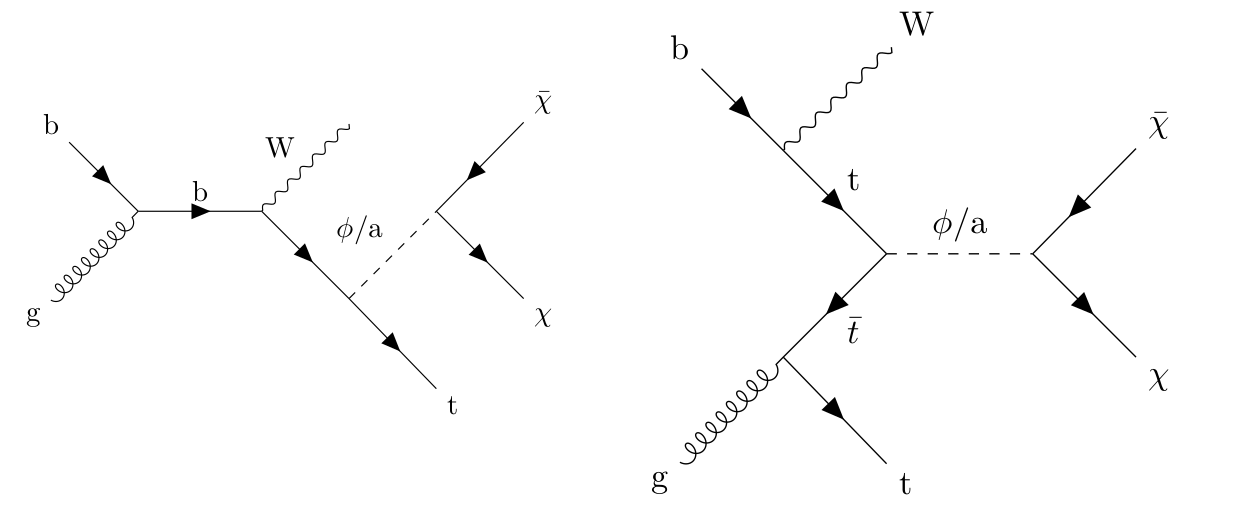
\includegraphics[width=1.0\textwidth]{figs/feynman_tDM_mine.png}
    		 \end{center}
	\end{column} \hfill
	\begin{column}{0.3\textwidth}
		\begin{center}
			\begin{block}{\centering $t \bar t$+DM model}\end{block}				
			%\alert{\textbf{$t \bar t$ + DM model}} \\ \vspace{5pt}
			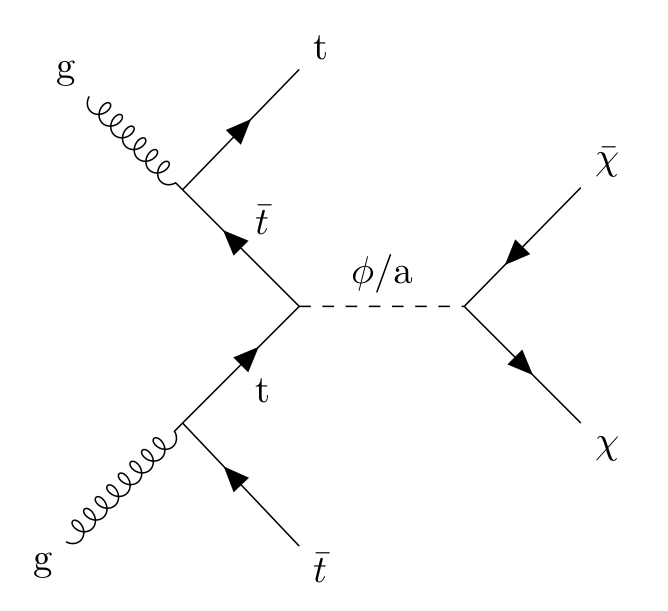
\includegraphics[width=1.0\textwidth]{figs/feynman_ttDM_mine.png}
    		 \end{center}
	\end{column} \hfill
\end{columns} \vfill

%The Yukawa coupling typically favors searches for dark matter \textbf{produced in association with heavy quarks} such as this one. Such MET+X are heavily depend on the MET spectrum, which is expected to be larger for the signals than most backgrounds. \vfill
\end{frame}

\begin{frame}{Focus of this analysis II}
\justifying
The \textbf{typical final state} of such models is made out of:
\begin{itemize}
\justifying
\item 1 or 2 b-tagged jets coming from the decay of the top quark(s);
\item 2 W bosons, seen as a combination of jets and leptons depending on the channel;
\item Some MET coming from the dark matter and the decay of the Ws;
\end{itemize} \vfill

In particular, we are studying the \alert{dilepton final state} in this work: 
\begin{itemize}
\justifying
\item Has the lowest branching ratio: BR($W \rightarrow l^+ + \nu_l) = (10.80 \pm 0.09)\%$ for each of the tree leptons (contains only $5\%$ of the signal events);
\item But, leptons can usually be reconstructed better than jets, resulting in lower systematic uncertainties;
\item And this channel also has the lowest number of backgrounds, resulting in a better signal isolation.
\end{itemize} \vfill

This channel is then \textbf{expected to be competitive with the hadronic channel}, especially when considering high mediator masses, which feature a higher global discrimination signal/background. \vfill
\end{frame}











%
%\begin{frame}[standout]
%Global strategy
%\end{frame}

\begin{frame}{Analysis strategy}
\justifying
Run II legacy paper being worked on, expected to \alert{combine both the $t/\bar t$+DM and $t \bar t$+DM searches}, and the 3 possible final states (hadronic, semi-leptonic and dileptonic). \\
\hspace{10pt} $\rightarrow$ Paper expected to be approved by LHCP ($\sim$ June). \vfill

The effort is \textbf{globally common} between the groups studying the different final states:
\begin{itemize}
\justifying
\item Objects are defined in a common way;
\item Control and signal region orthogonal between the channels.
\begin{itemize}
\justifying
\item Number of leptons and b-jet categorization to improve the sensitivity by defining enriched $t/\bar t$+DM/$t \bar t$+DM regions.
\end{itemize}
\end{itemize} \vfill

This talk will \textbf{be focused on the dilepton final state}, in which we are mostly involved, along with a team of DESY. Deborah Pinna and her team from the University of Wisconsin are focused on the semi-leptonic and hadronic channels. \vfill
\end{frame}

\begin{frame}{Framework used}
\justifying
This analysis \textbf{almost entirely relies on the Latino framework}:

\begin{itemize}
\justifying
\item We use the usual Latino objects;
\item We produced our own signal trees privately, stored in our own eos directories given the tight space available in the HWW directory;
\item A custom post-processing step was run on top of the l2tight trees, in order to:

\begin{itemize}
\justifying
\item Perform a general Betchart reconstruction of the $t \bar t$ system;
\item Skim the trees;
\item Compute and store additional variables, such as the number o medium deepCSV b-jets or the stranverse mass $m_{T2}^{ll}$ as used in EXO.
\end{itemize}
\end{itemize} \vfill

A custom setup made in PlotsConfigurations was then used to plot the results and produce the datacards needed. \vfill
In general, the process was really smooth given the reliability of the framework in general and the high number of scripts available, able to perform a lot of different taks. \vfill
\end{frame}


























\begin{frame}[standout]
Inclusive selection
\end{frame}

\begin{frame}{Inclusive selection}
\justifying
\vspace{5pt}
\begin{block}{\centering Inclusive selection}\end{block} \vfill
\vspace{-5pt}

First, distributions in the following inclusive control region mostly enriched in Drell-Yan were studied, in all the different channels available:
\begin{itemize}
\item Leading (trailing) lepton $p_T >$ 25 (20) GeV
\item Third lepton veto ($p_T < 10$ GeV)
\item Opposite sign leptons
\item $m_{ll} > 20$ GeV to avoid low mass resonances
\item At least 1 jet
\item At least 1 medium deep CSV b-jet
\end{itemize} \vfill

This region is studied to have a look at the most inclusive selection to spot initial issues and problems. \vfill

A slight mismodeling of the low mass DY+Jets sample and a general problem of the MET in DY events is observed, but these features are known in CMS and are mitigated with the analysis cuts applied. \vfill
\end{frame}

%\begin{frame}{Control regions}
%\vspace{5pt}
%\begin{block}{\centering Control regions}\end{block} \vfill
%\vspace{-5pt}
%\begin{itemize}
%\item An \alert{inclusive} region:
%\vspace{-10pt}
%\begin{multicols}{2}
%\begin{itemize}
%\item First 2 tight leptons: $p_T > 25, 20$ GeV
%\item Third lepton: $p_T < 10$ GeV
%\item Opposite sign leptons
%\item $m_{ll} > 20$ GeV
%\item At least 1 jet
%\item At least 1 b-jet
%\end{itemize}
%\end{multicols} \vfill
%
%\item A \alert{Drell-Yan} CR, defined as the inclusive region and:
%\vspace{-10pt}
%\begin{multicols}{2}
%\begin{itemize}
%\item 15 GeV Z window ($ee$/$\mu \mu$ channels)
%\item $M_{T2}^{ll} > 80$ GeV
%\end{itemize}
%\end{multicols} \vfill
%
%\item A \alert{$t \bar t$} CR, similar to the $t \bar t$ + DM signal region but with $60 < M_{T2}(ll) < 80$ GeV \vfill \vspace{10pt}
%
%\item A \alert{ttV} (ttW + ttZ) enriched CR:
%\vspace{-10pt}
%\begin{multicols}{2}
%\begin{itemize}
%\item At least 3 tight leptons
%\item $M_{T2}^{ll} > 80$ GeV
%\end{itemize}
%\end{multicols} \vfill
%
%\item A \alert{same-sign CR} for the non-prompt background:
%\vspace{-10pt}
%\begin{multicols}{2}
%\begin{itemize}
%\item Inclusive selection but with same sign leptons
%\item 15 GeV Z-veto ($ee$/$\mu \mu$ channels)
%\end{itemize}
%\end{multicols} \vfill
%\end{itemize}
%\end{frame}

\begin{frame}{Inclusive control region}
\begin{columns}
\begin{column}{1.09\textwidth}
\begin{block}{\centering $ll$ channel}\end{block}
\end{column}
\end{columns} \vspace{-5pt}
\begin{columns}
		\begin{column}{0.33\textwidth}
			\begin{center}
			\vspace{-8pt}
			\begin{block}{\centering 2016}\end{block}\vspace{10pt}
     			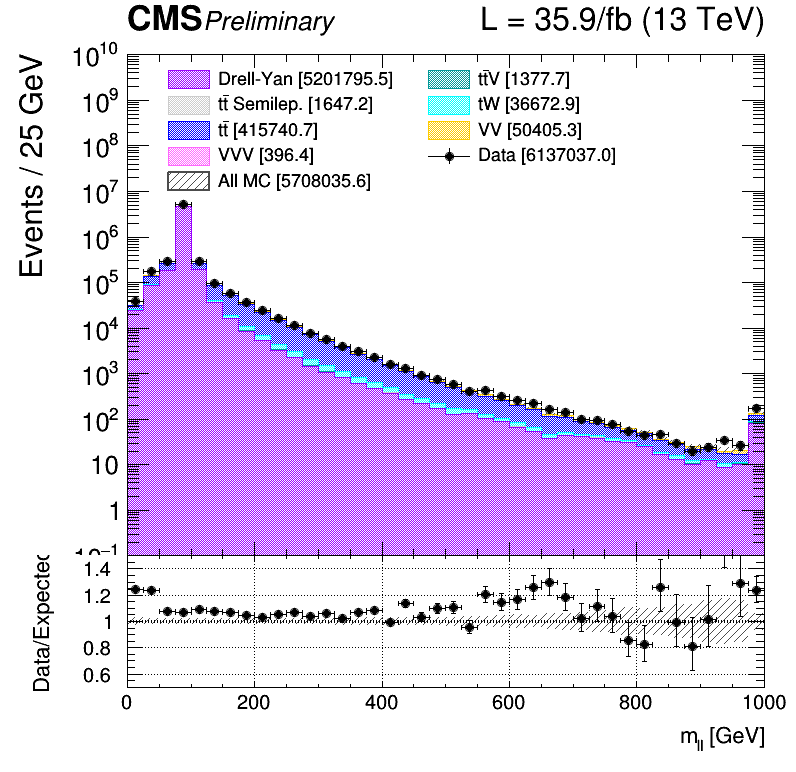
\includegraphics[width=1.0\textwidth, height=90pt]{figs/2016/log_cratio_inclusiveCR_ll_mll.png}
    		\end{center}		
		\end{column} 
		\begin{column}{0.33\textwidth}
			\begin{center}
			\vspace{-8pt}
			\begin{block}{\centering 2017}\end{block}\vspace{10pt}
     			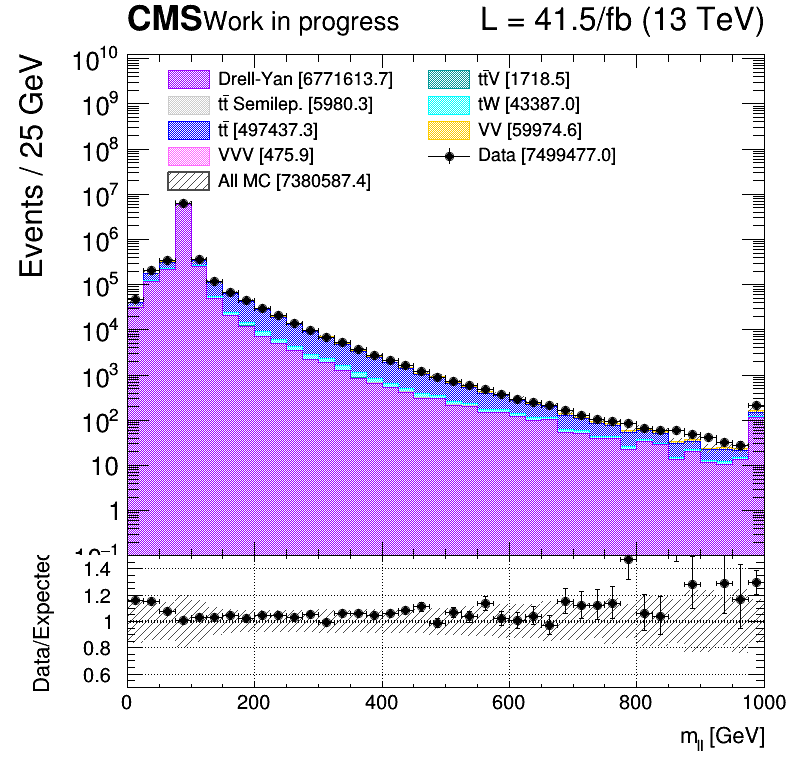
\includegraphics[width=1.0\textwidth, height=90pt]{figs/2017/log_cratio_inclusiveCR_ll_mll.png}
    		\end{center}		
		\end{column} 
		\begin{column}{0.33\textwidth}
			\begin{center}
			\vspace{-8pt}
			\begin{block}{\centering 2018}\end{block}\vspace{10pt}
     			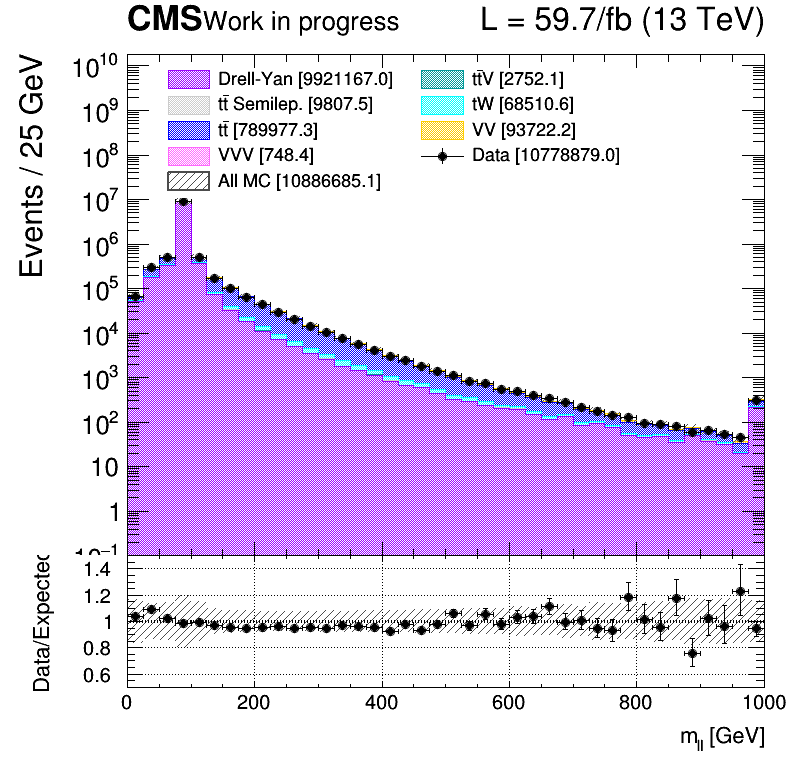
\includegraphics[width=1.0\textwidth, height=90pt]{figs/2018/log_cratio_inclusiveCR_ll_mll.png}
    		\end{center}		
		\end{column}
\end{columns}
\begin{columns}
		\begin{column}{0.33\textwidth}
			\begin{center}
				%\begin{block}{\centering Puppi MET}\end{block}	
     			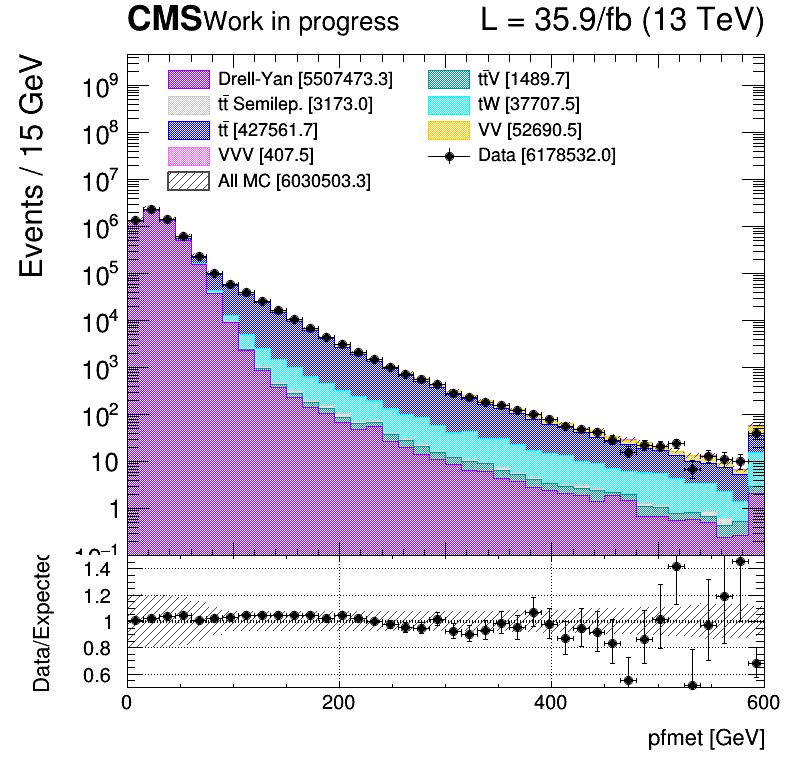
\includegraphics[width=1.0\textwidth, height=90pt]{figs/2016/log_cratio_inclusiveCR_ll_METcorrected_pt.png}
    		\end{center}		
		\end{column}
		\begin{column}{0.33\textwidth}
			\begin{center}
				%\begin{block}{\centering njet}\end{block}	
     			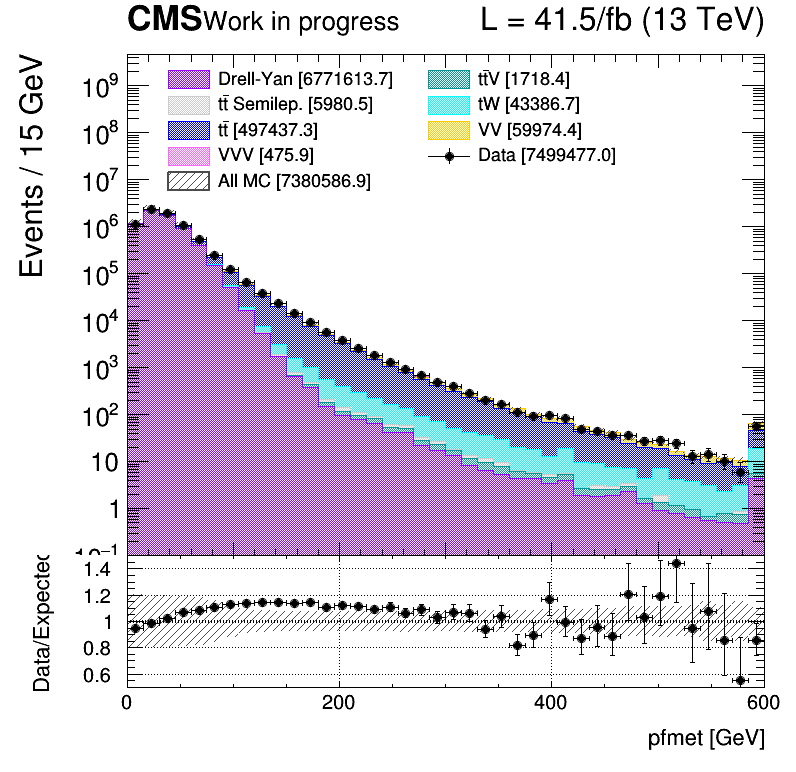
\includegraphics[width=1.0\textwidth, height=90pt]{figs/2017/log_cratio_inclusiveCR_ll_METcorrected_pt.png}
    		\end{center}		
		\end{column}
		\begin{column}{0.33\textwidth}
			\begin{center}
				%\begin{block}{\centering nbjet}\end{block}	
     			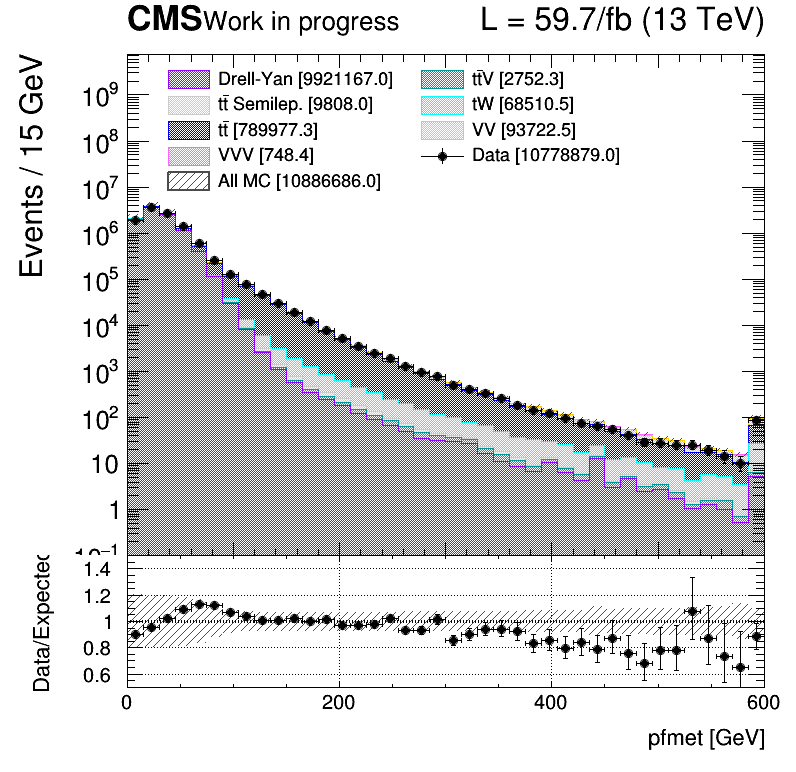
\includegraphics[width=1.0\textwidth, height=90pt]{figs/2018/log_cratio_inclusiveCR_ll_METcorrected_pt.png}
    		\end{center}		
		\end{column}
\end{columns} \vfill
\end{frame}

\begin{frame}{Inclusive control region}
\begin{columns}
\begin{column}{1.09\textwidth}
\begin{block}{\centering df channel}\end{block}
\end{column}
\end{columns} \vspace{-5pt}
\begin{columns}
		\begin{column}{0.33\textwidth}
			\begin{center}
			\vspace{-8pt}
			\begin{block}{\centering 2016}\end{block}\vspace{10pt}
     			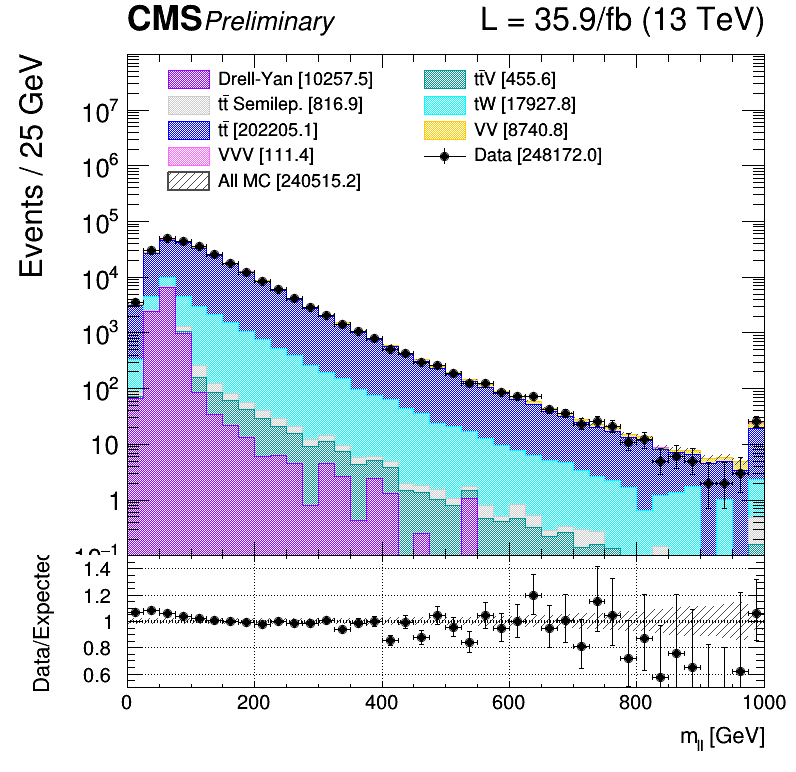
\includegraphics[width=1.0\textwidth, height=90pt]{figs/2016/log_cratio_inclusiveCR_df_mll.png}
    		\end{center}		
		\end{column} 
		\begin{column}{0.33\textwidth}
			\begin{center}
			\vspace{-8pt}
			\begin{block}{\centering 2017}\end{block}\vspace{10pt}
     			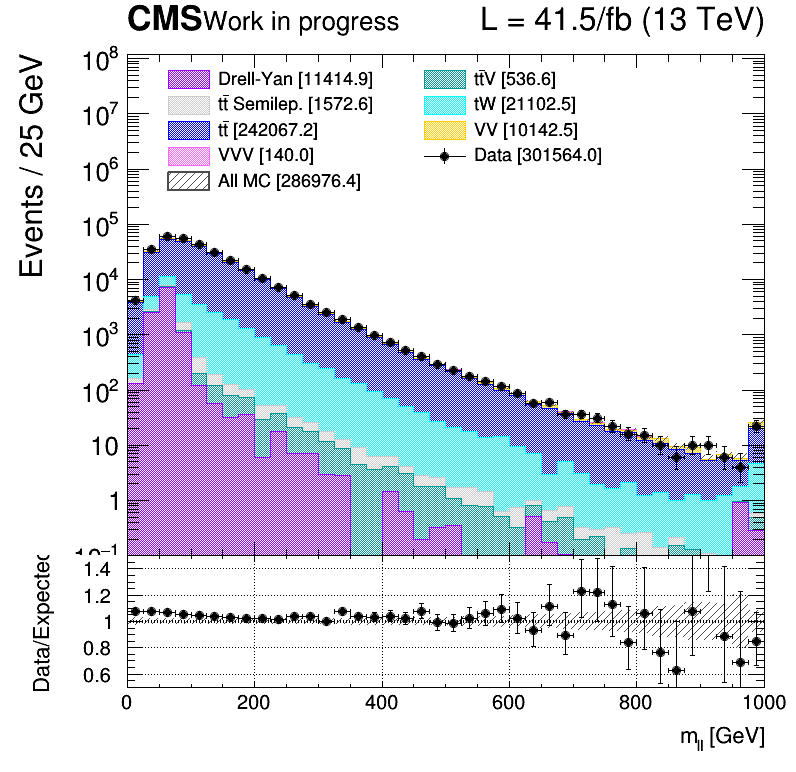
\includegraphics[width=1.0\textwidth, height=90pt]{figs/2017/log_cratio_inclusiveCR_df_mll.png}
    		\end{center}		
		\end{column} 
		\begin{column}{0.33\textwidth}
			\begin{center}
			\vspace{-8pt}
			\begin{block}{\centering 2018}\end{block}\vspace{10pt}
     			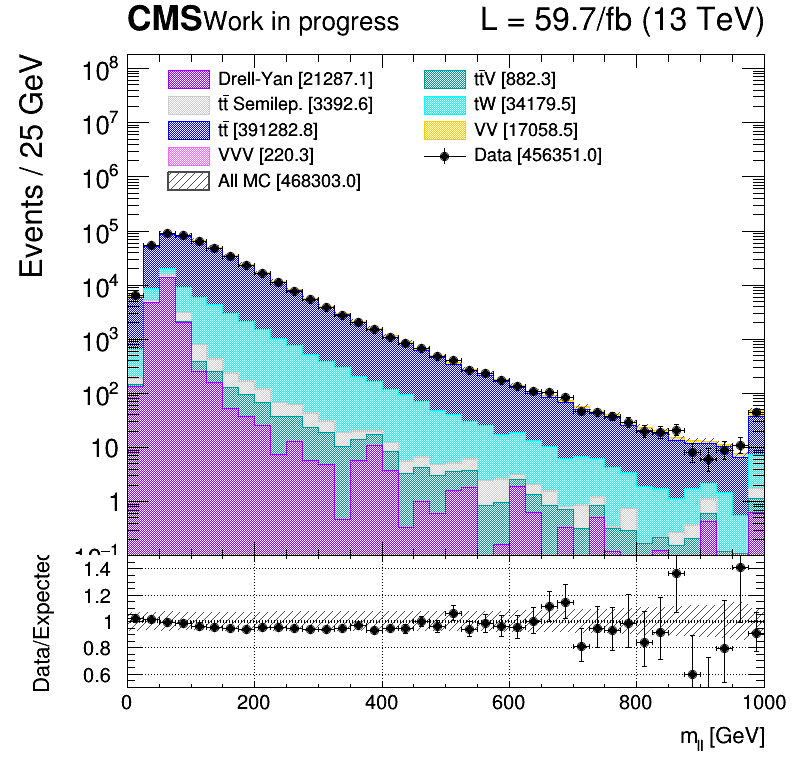
\includegraphics[width=1.0\textwidth, height=90pt]{figs/2018/log_cratio_inclusiveCR_df_mll.png}
    		\end{center}		
		\end{column}
\end{columns}
\begin{columns}
		\begin{column}{0.33\textwidth}
			\begin{center}
				%\begin{block}{\centering Puppi MET}\end{block}	
     			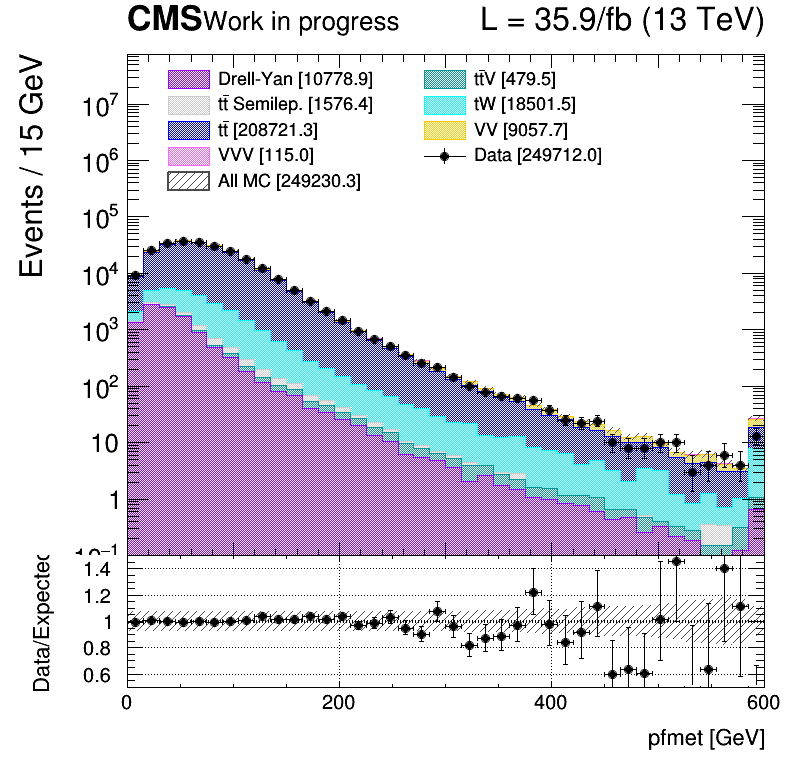
\includegraphics[width=1.0\textwidth, height=90pt]{figs/2016/log_cratio_inclusiveCR_df_METcorrected_pt.png}
    		\end{center}		
		\end{column}
		\begin{column}{0.33\textwidth}
			\begin{center}
				%\begin{block}{\centering njet}\end{block}	
     			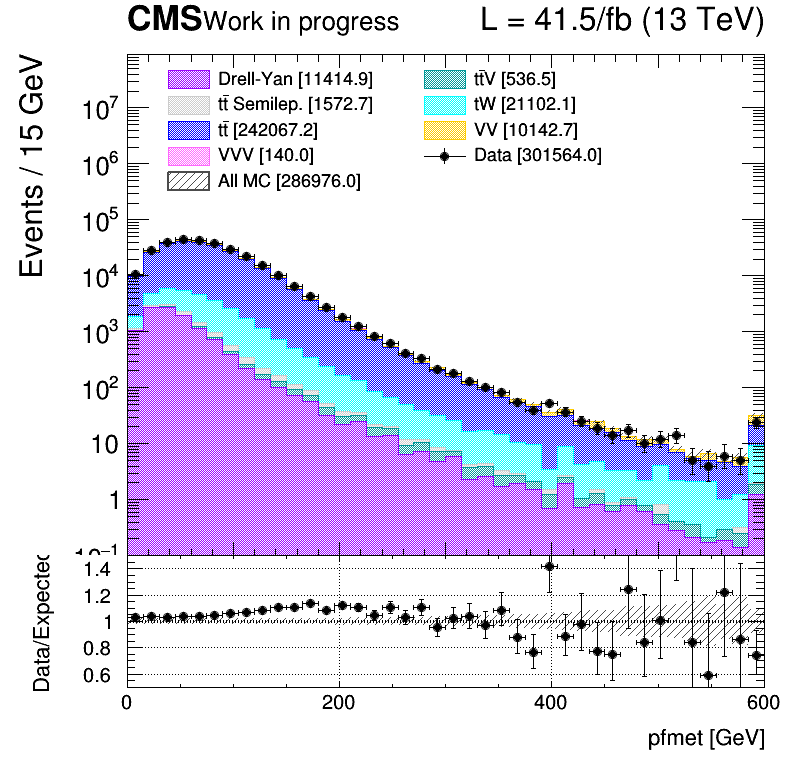
\includegraphics[width=1.0\textwidth, height=90pt]{figs/2017/log_cratio_inclusiveCR_df_METcorrected_pt.png}
    		\end{center}		
		\end{column}
		\begin{column}{0.33\textwidth}
			\begin{center}
				%\begin{block}{\centering nbjet}\end{block}	
     			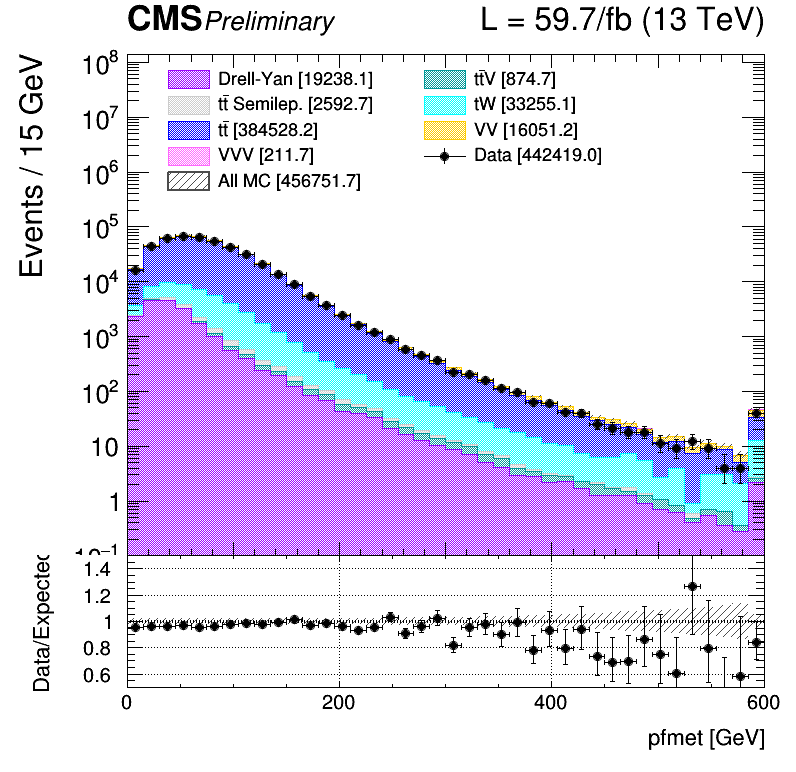
\includegraphics[width=1.0\textwidth, height=90pt]{figs/2018/log_cratio_inclusiveCR_df_METcorrected_pt.png}
    		\end{center}		
		\end{column}
\end{columns} \vfill
\end{frame}






















\begin{frame}[standout]
Signal extraction
\end{frame}

\begin{frame}{MVA training}
\justifying
We \alert{trained an ANN}, featuring the following characteristics:
\vspace{-5pt}
\begin{itemize}
\justifying
\item 80/80/40 hidden neurons
\item Mix of standard model $t \bar t$ and single top as \textbf{backgrounds}, and mix of both $t/\bar t$+DM and $t \bar t$+DM as \textbf{signals};
\item Only events passing the \textbf{following pre-selection} are considered for the training:
\vspace{-10pt}
\begin{multicols}{2}
\begin{itemize}
\item 2 tight leptons: $p_T > 25, 20$ GeV
\item Third lepton: $p_T < 10$ GeV
\item Opposite sign leptons
\item $m_{ll} > 20$ GeV
\item 15 GeV Z-veto in $ee$ and $\mu \mu$ channels
\item At least 1 jet
\item At least 1 b-jet
\item $M_{T2}^{ll} > 80$ GeV, to stay orthogonal to the other channels
\end{itemize}
\end{multicols} 
\vspace{-10pt}
\item One specific training performed per signal mass point;
\item 50\% train/test splitting used ($\sim 40.000$ training events in total).
\end{itemize} \vfill

The ANN shape obtained is used to perform a general \alert{shape analysis}. \vfill

The TMVA package was then finally used to study the training performed, as shown in the next few slides for the 2016 scalar 100/500GeV training performed. We plan on combining all the year together. \vfill	
\end{frame}

\begin{frame}{2018 discriminating variables}
Example distributions shown in the blinded 2018 pre-selection region. \vfill
\begin{columns}
\begin{column}{1.09\textwidth}
\begin{block}{\centering 2018, $ll$ channel}\end{block} \vspace{10pt}
\end{column}
\end{columns} \vspace{-5pt}
\begin{columns}
		\begin{column}{0.33\textwidth}
			\begin{center}
     			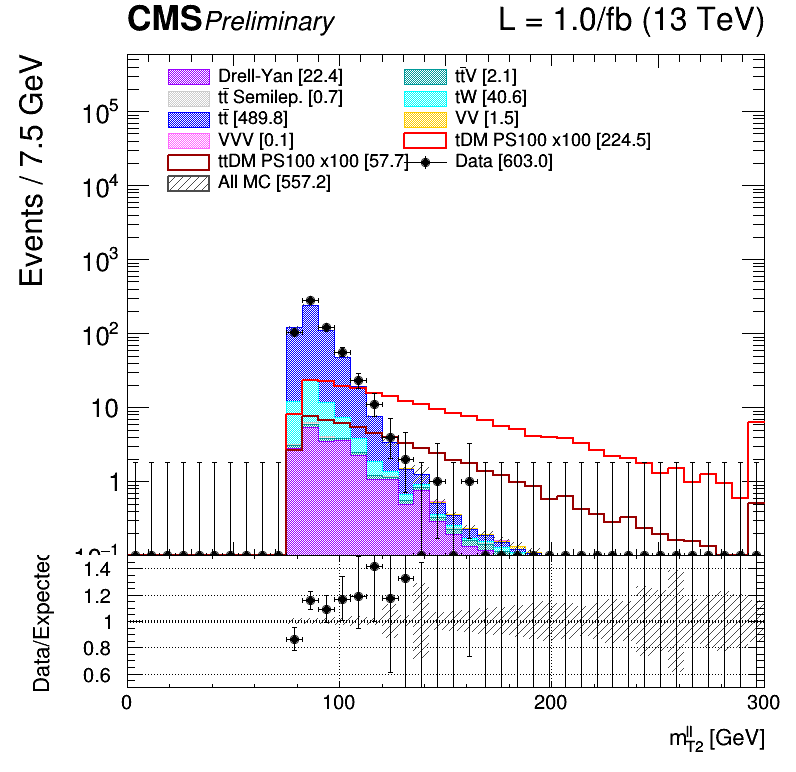
\includegraphics[width=1.0\textwidth, height=90pt]{figs/2018/log_cratio_topCR_ll_mt2ll.png}
    		\end{center}		
		\end{column} 
		\begin{column}{0.33\textwidth}
			\begin{center}
     			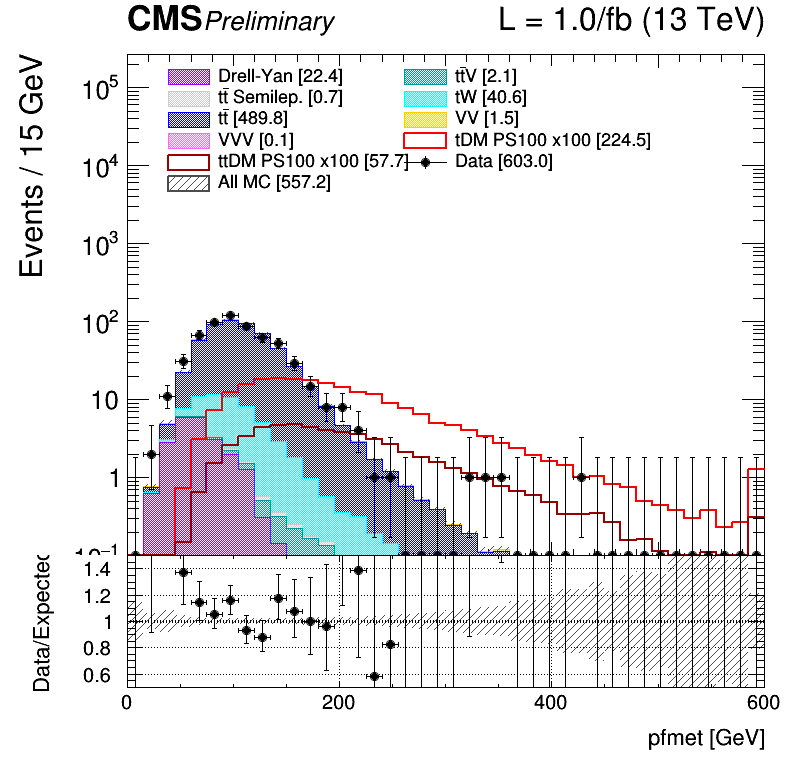
\includegraphics[width=1.0\textwidth, height=90pt]{figs/2018/log_cratio_topCR_ll_METcorrected_pt.png}
    		\end{center}		
		\end{column} 
		\begin{column}{0.33\textwidth}
			\begin{center}
     			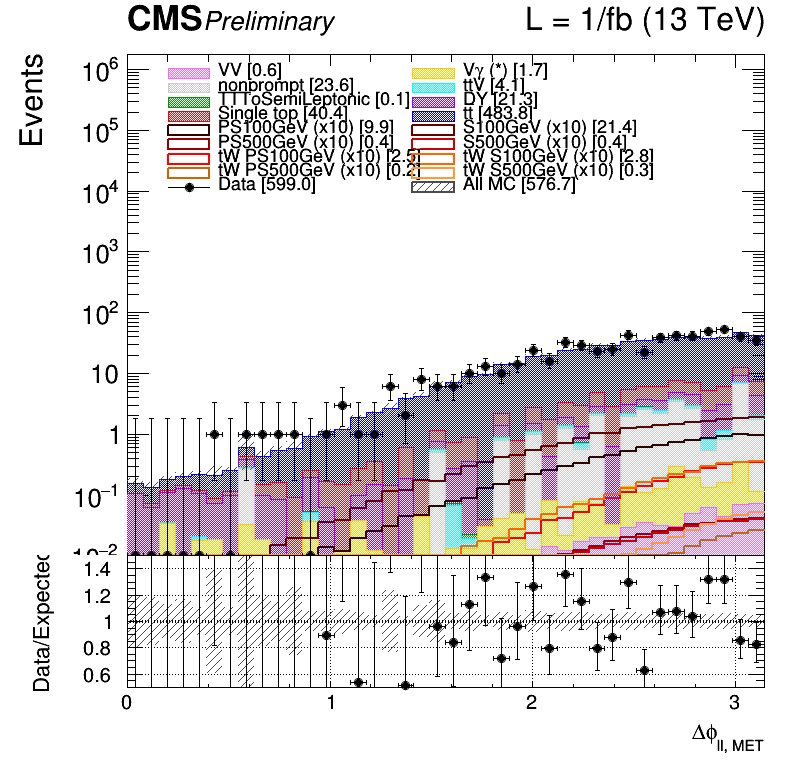
\includegraphics[width=1.0\textwidth, height=90pt]{figs/2018/log_cratio_topCR_ll_dphillmet.png}
    		\end{center}		
		\end{column}
\end{columns}
\begin{columns}
		\begin{column}{0.33\textwidth}
			\begin{center}
				%\begin{block}{\centering Puppi MET}\end{block}	
     			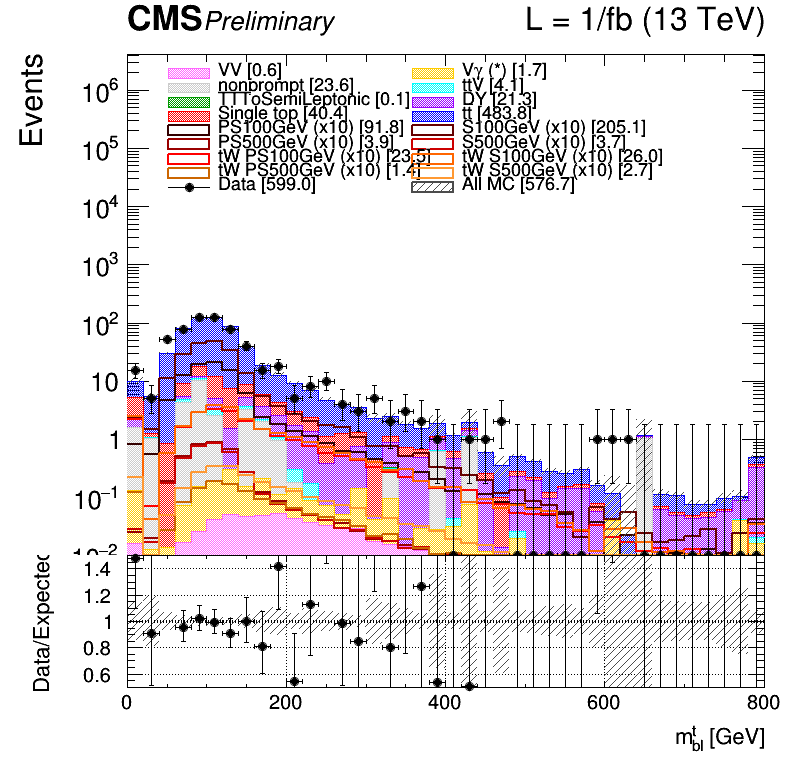
\includegraphics[width=1.0\textwidth, height=90pt]{figs/2018/log_cratio_topCR_ll_mblt.png}
    		\end{center}		
		\end{column}
		\begin{column}{0.33\textwidth}
			\begin{center}
				%\begin{block}{\centering njet}\end{block}	
     			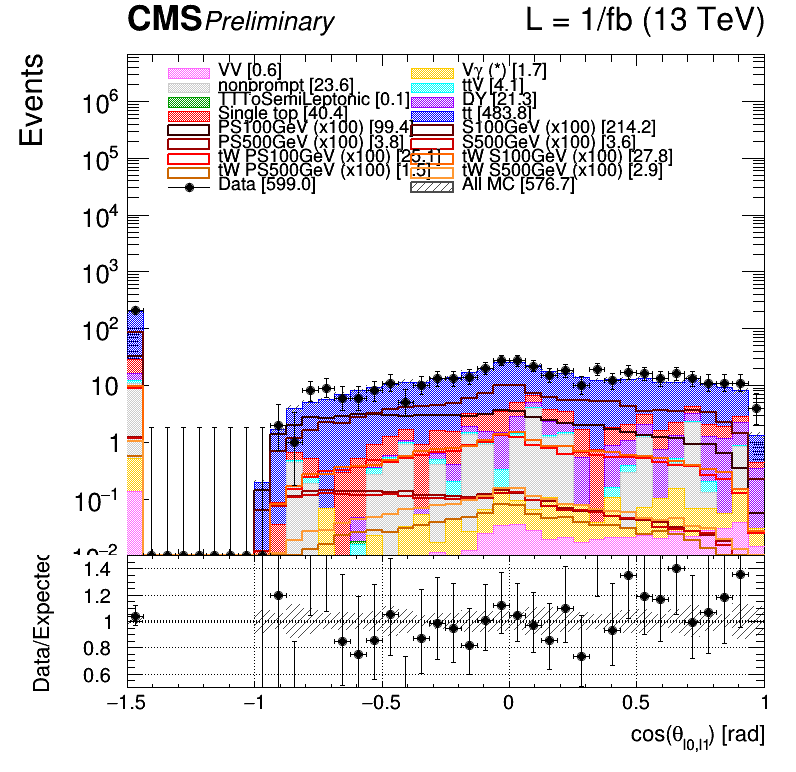
\includegraphics[width=1.0\textwidth, height=90pt]{figs/2018/log_cratio_topCR_ll_costhetall.png}
    		\end{center}		
		\end{column}
		\begin{column}{0.33\textwidth}
			\begin{center}
				%\begin{block}{\centering nbjet}\end{block}	
     			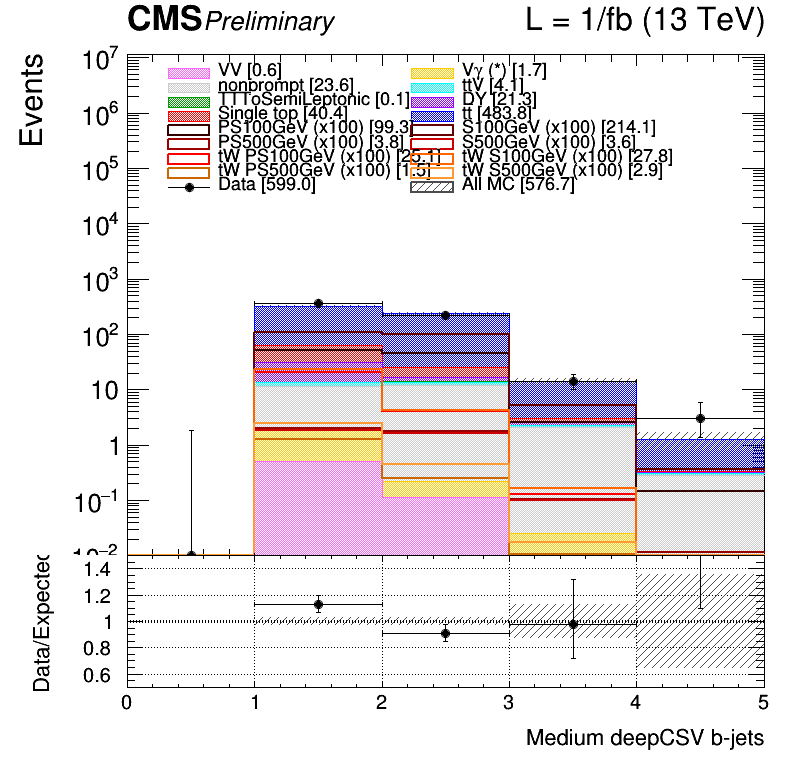
\includegraphics[width=1.0\textwidth, height=90pt]{figs/2018/log_cratio_topCR_ll_nbjet.png}
    		\end{center}		
		\end{column}
\end{columns} \vfill
\end{frame}

\begin{frame}{ROC curves}
\justifying
%\begin{block}{\centering Scalar mediators}\end{block} \vspace{-10pt}
ROC curves have been obtained for all the different mass points available, from 50 to 500 GeV, and for both scalar and pseudoscalar mediators. \vfill
\begin{figure}[htbp]
\centering
\begin{minipage}[b]{.49\textwidth}
\vspace{-5pt}
\begin{block}{\centering Scalar mediator}\end{block}
\begin{center}
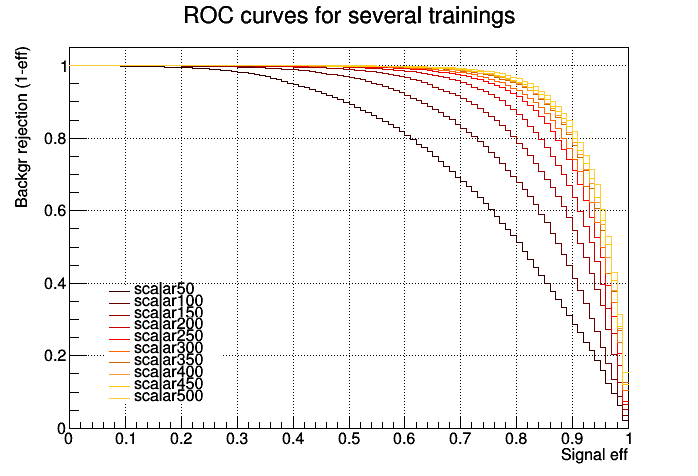
\includegraphics[width=5.2cm, height=3.5cm]{figs/groupedROC_scalar.png}
\end{center}
\end{minipage}
\begin{minipage}[b]{.02\textwidth}\end{minipage}
\begin{minipage}[b]{.49\textwidth}
\vspace{-5pt}
\begin{block}{\centering Pseudoscalar mediator}\end{block}
\begin{center}
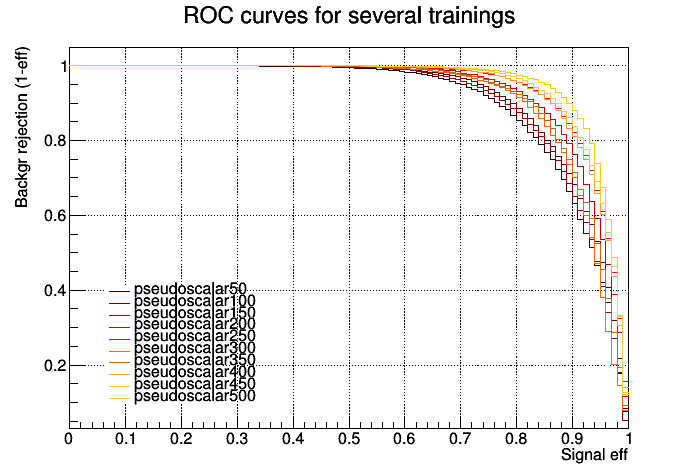
\includegraphics[width=5.2cm, height=3.5cm]{figs/groupedROC_pseudo.png}
\end{center}
\end{minipage}
\end{figure} \vfill
As expected, a better discrimination is achieved for higher mediator masses. \vfill
\end{frame}

\begin{frame}{Blinded ANN output shape}
\begin{columns}
\begin{column}{1.09\textwidth}
\begin{block}{\centering Scalar 100 GeV output shape}\end{block}
\end{column}
\end{columns} \vspace{-5pt}

\begin{columns}
		\begin{column}{0.33\textwidth}
			\begin{center}
			\vspace{-8pt}
			\begin{block}{\centering 2016}\end{block}
     			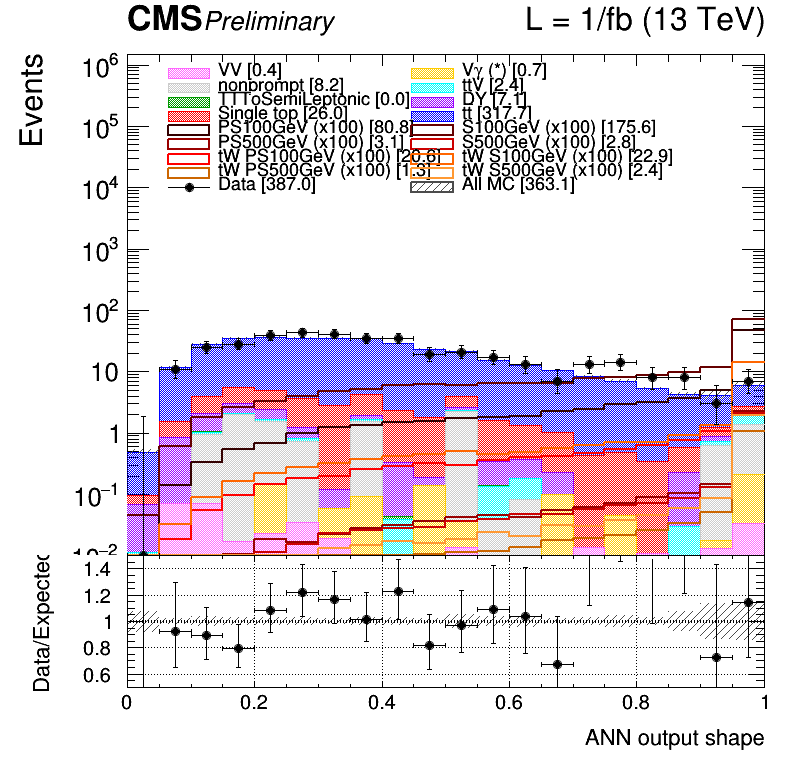
\includegraphics[width=1.0\textwidth, height=90pt]{figs/2016/log_cratio_topCR_ll_var_DNN_signal0_scalar100.png}
    		\end{center}		
		\end{column} 
		\begin{column}{0.33\textwidth}
			\begin{center}
			\vspace{-8pt}
			\begin{block}{\centering 2017}\end{block}
     			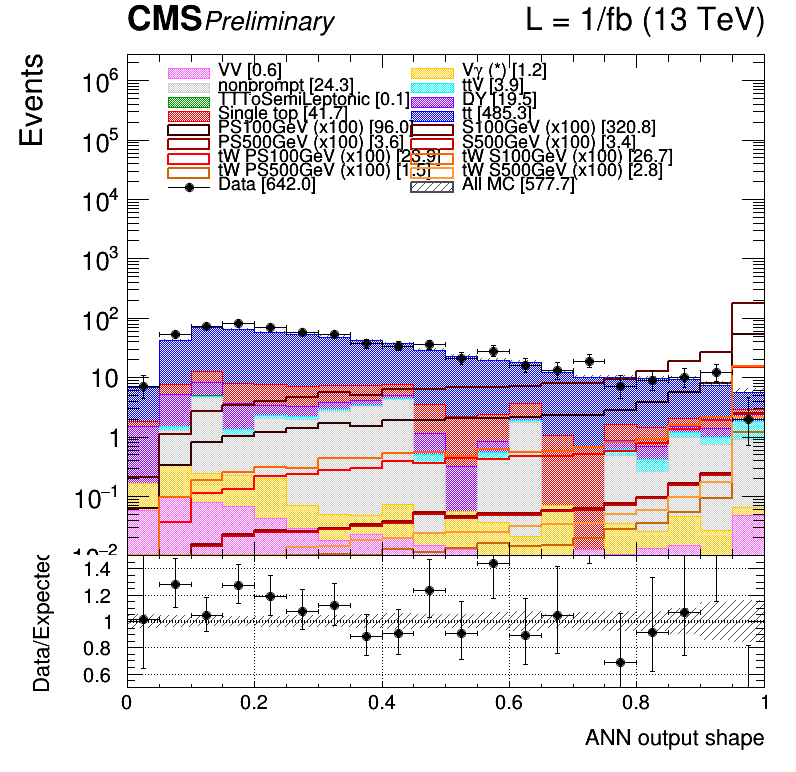
\includegraphics[width=1.0\textwidth, height=90pt]{figs/2017/log_cratio_topCR_ll_var_DNN_signal0_scalar100.png}
    		\end{center}		
		\end{column} 
		\begin{column}{0.33\textwidth}
			\begin{center}
			\vspace{-8pt}
			\begin{block}{\centering 2018}\end{block}
     			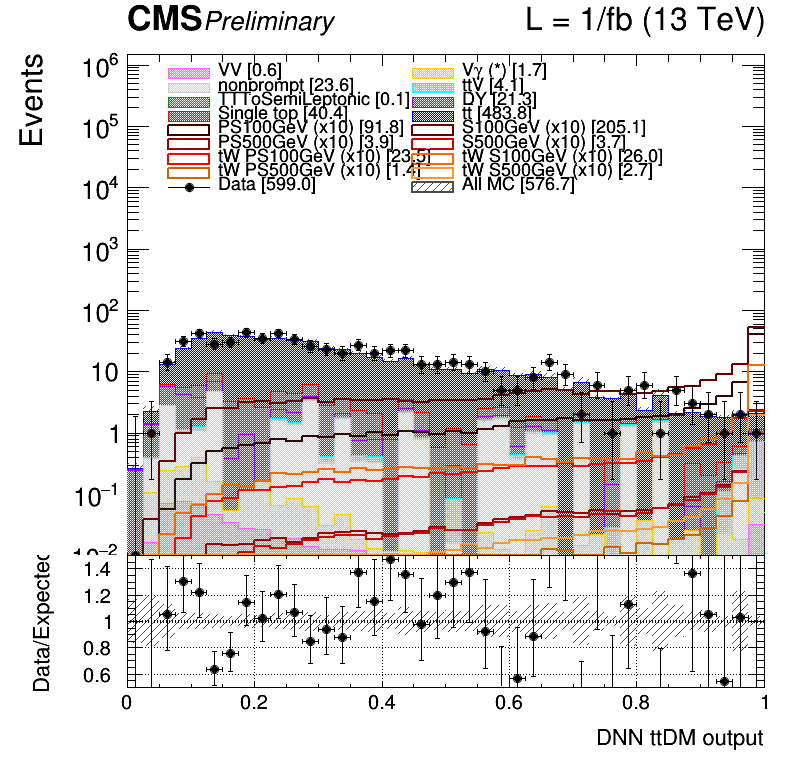
\includegraphics[width=1.0\textwidth, height=90pt]{figs/2018/log_cratio_topCR_ll_var_DNN_signal0_scalar100.png}
    		\end{center}		
		\end{column}
\end{columns}

\begin{columns}
\begin{column}{1.09\textwidth}
\begin{block}{\centering Scalar 500 GeV output shape}\end{block}
\end{column}
\end{columns} \vspace{-5pt}
\begin{columns}
		\begin{column}{0.33\textwidth}
			\begin{center}
				%\begin{block}{\centering Puppi MET}\end{block}	
     			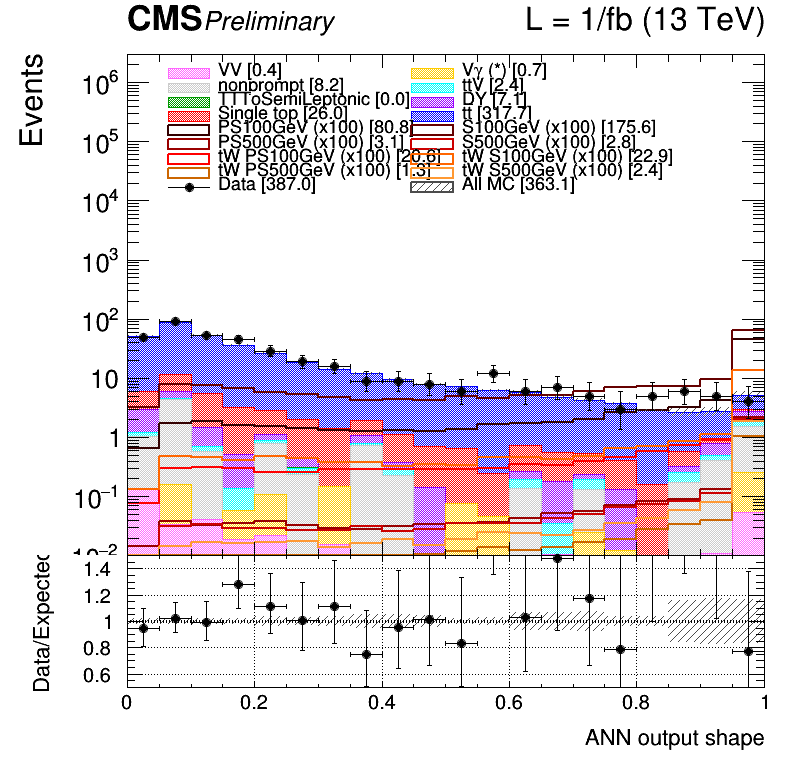
\includegraphics[width=1.0\textwidth, height=90pt]{figs/2016/log_cratio_topCR_ll_var_DNN_signal0_scalar500.png}
    		\end{center}		
		\end{column}
		\begin{column}{0.33\textwidth}
			\begin{center}
				%\begin{block}{\centering njet}\end{block}	
     			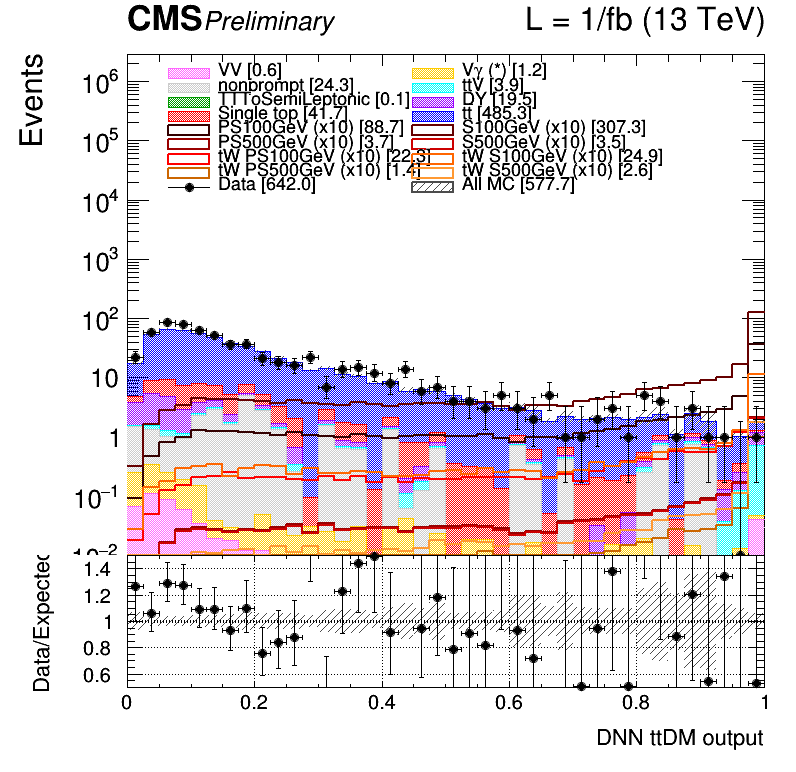
\includegraphics[width=1.0\textwidth, height=90pt]{figs/2017/log_cratio_topCR_ll_var_DNN_signal0_scalar500.png}
    		\end{center}		
		\end{column}
		\begin{column}{0.33\textwidth}
			\begin{center}
				%\begin{block}{\centering nbjet}\end{block}	
     			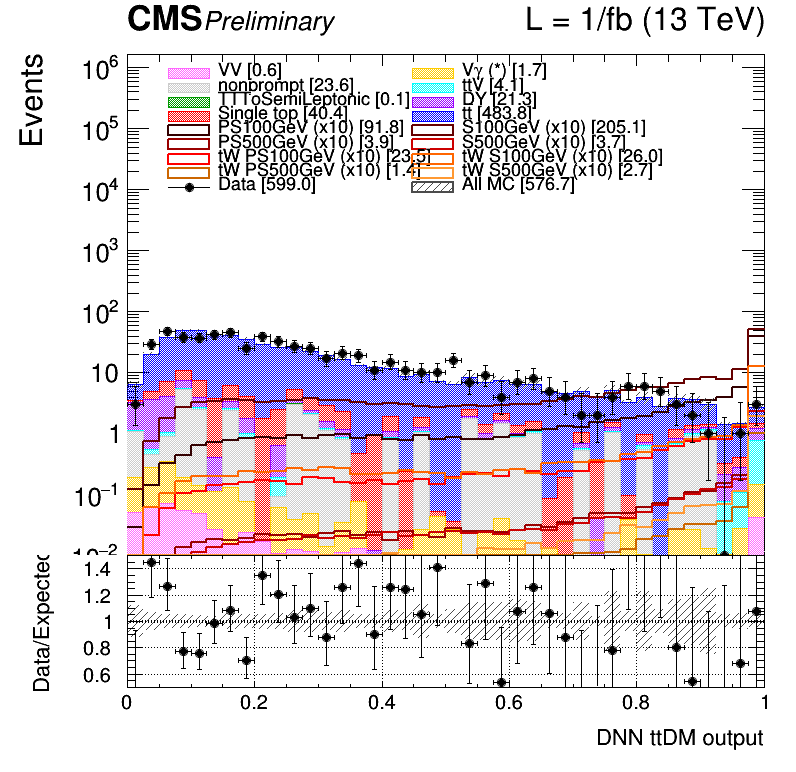
\includegraphics[width=1.0\textwidth, height=90pt]{figs/2018/log_cratio_topCR_ll_var_DNN_signal0_scalar500.png}
    		\end{center}		
		\end{column}
\end{columns} \vfill
\end{frame}











































\begin{frame}[standout]
Background prediction methods
\end{frame}

\begin{frame}{Main background processes}
\justifying
The backgrounds are predicted either directly from \alert{Monte-Carlo simulations or from data-driven methods}. In order of importance:

\begin{itemize}
\justifying
\item The \textbf{$t \bar t$ and the single top} are taken from simulation accounting for all the variations in the generation parameters. Several parameters (QCD scale, PDF variation,...) are varied and included as a systematic (see later). \\
$\rightarrow$ A data validation region (low $M_{T2}^{ll}$) is explored to ensure the quality of the prediction;
\item The \textbf{Drell-Yan} yields are obtained from a semi data-driven method using the excluded same flavor region on the Z peak as control region;
\item The \textbf{non-prompt contamination} is estimated from data control regions and validated in a same sign validation region;
\item The irreducible \textbf{ttV process} (ttW + ttZ) is taken from simulation and checked in a particular validation region;
\item \textbf{Diboson processes and other minor backgrounds} are taken directly from MC.
\end{itemize}
\end{frame}

\begin{frame}{Top control region}
\justifying
Same as the signal region but with $60 < M_{T2}^{ll} < 80$ GeV. \vfill

\begin{columns}
\begin{column}{1.09\textwidth}
\begin{block}{\centering $ll$ channel}\end{block}
\end{column}
\end{columns} \vspace{-5pt}

\begin{columns}
		\begin{column}{0.33\textwidth}
			\begin{center}
			\vspace{-8pt}
			\begin{block}{\centering 2016}\end{block}\vspace{10pt}
     			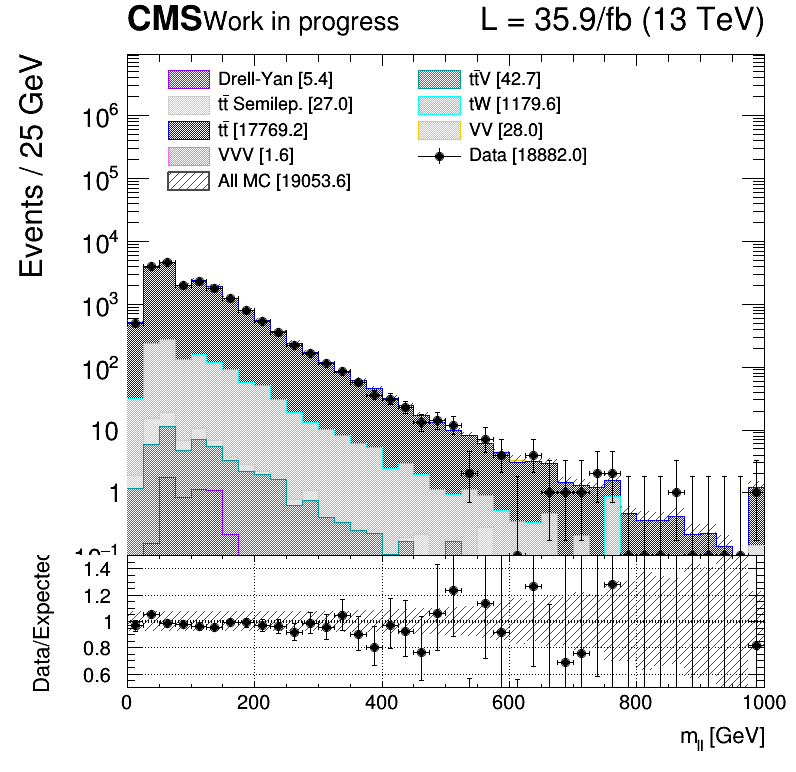
\includegraphics[width=1.0\textwidth, height=90pt]{figs/2016/log_cratio_ttbarCR_ll_mll.png}
    		\end{center}		
		\end{column} 
		\begin{column}{0.33\textwidth}
			\begin{center}
			\vspace{-8pt}
			\begin{block}{\centering 2017}\end{block}\vspace{10pt}
     			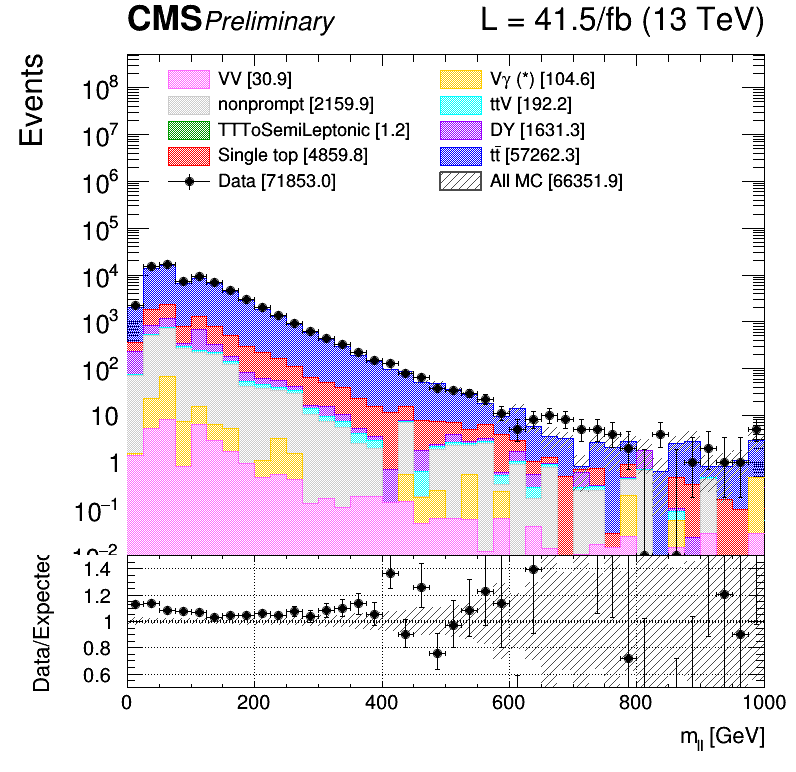
\includegraphics[width=1.0\textwidth, height=90pt]{figs/2017/log_cratio_ttbarCR_ll_mll.png}
    		\end{center}		
		\end{column} 
		\begin{column}{0.33\textwidth}
			\begin{center}
			\vspace{-8pt}
			\begin{block}{\centering 2018}\end{block}\vspace{10pt}
     			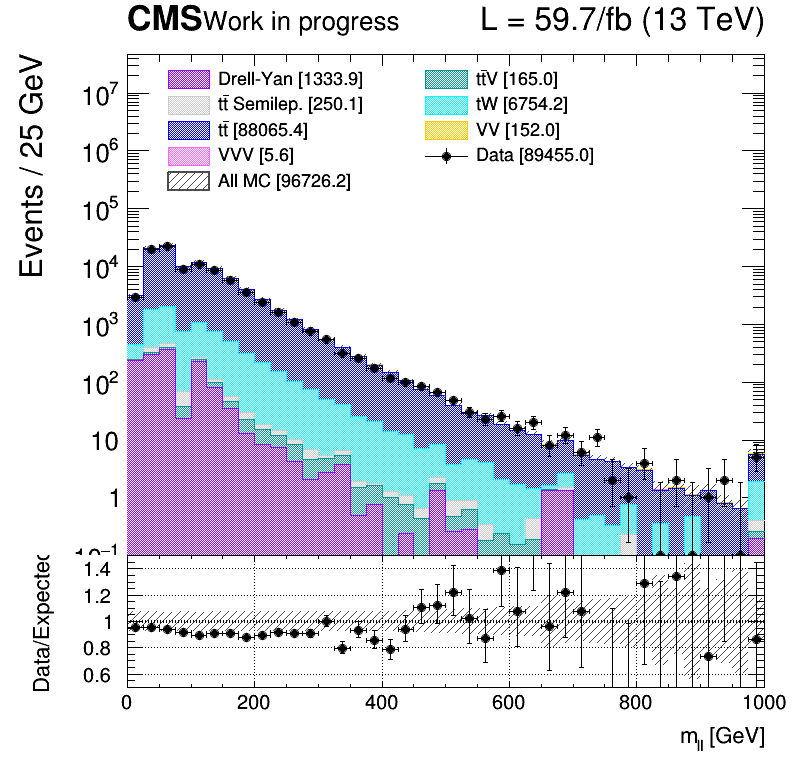
\includegraphics[width=1.0\textwidth, height=90pt]{figs/2018/log_cratio_ttbarCR_ll_mll.png}
    		\end{center}		
		\end{column}
\end{columns} \vspace{-10pt}
\begin{columns}
		\begin{column}{0.33\textwidth}
			\begin{center}
				%\begin{block}{\centering Puppi MET}\end{block}	
     			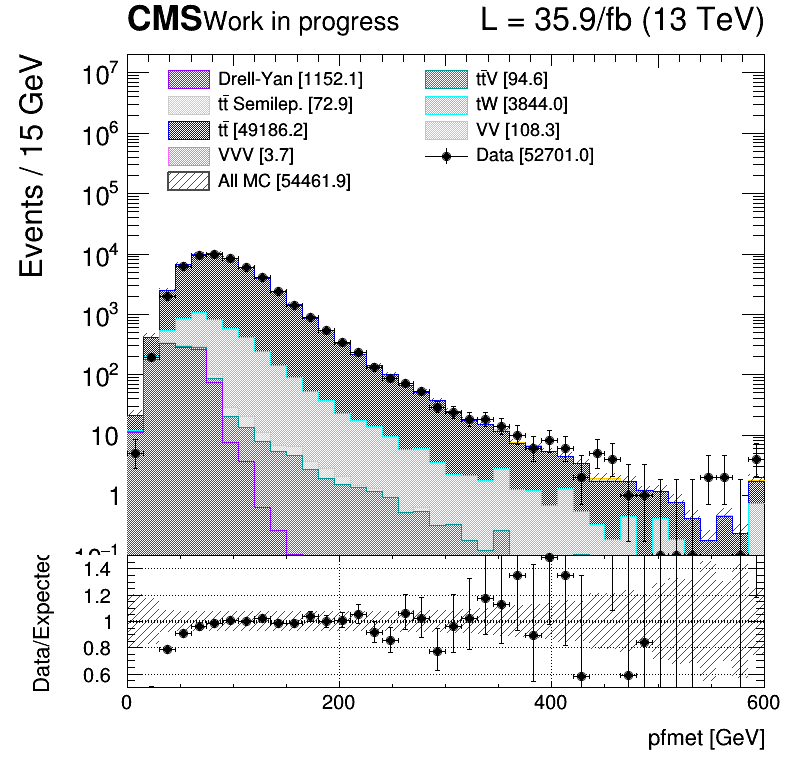
\includegraphics[width=1.0\textwidth, height=90pt]{figs/2016/log_cratio_ttbarCR_ll_METcorrected_pt.png}
    		\end{center}		
		\end{column}
		\begin{column}{0.33\textwidth}
			\begin{center}
				%\begin{block}{\centering njet}\end{block}	
     			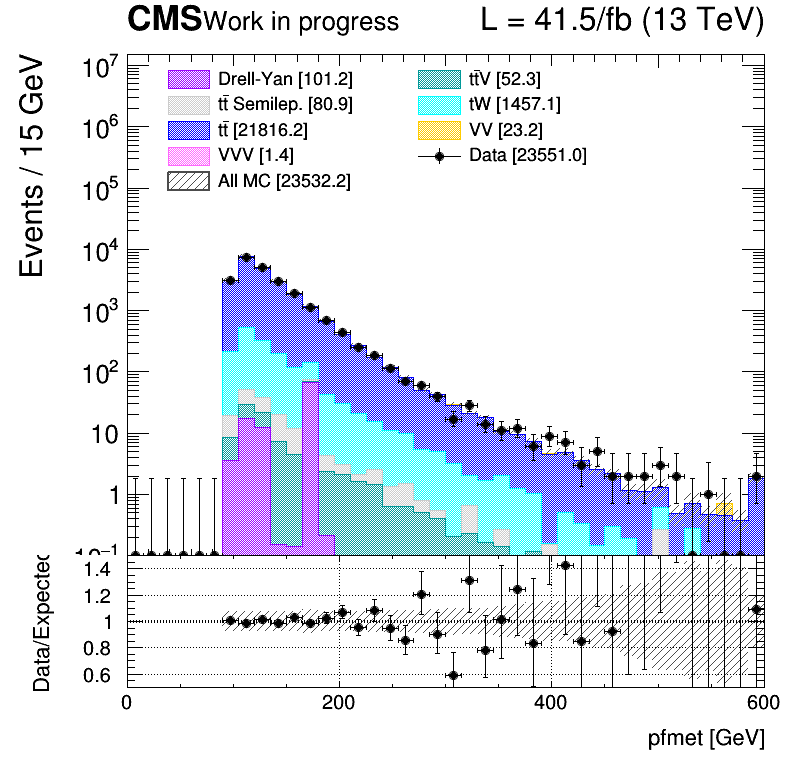
\includegraphics[width=1.0\textwidth, height=90pt]{figs/2017/log_cratio_ttbarCR_ll_METcorrected_pt.png}
    		\end{center}		
		\end{column}
		\begin{column}{0.33\textwidth}
			\begin{center}
				%\begin{block}{\centering nbjet}\end{block}	
     			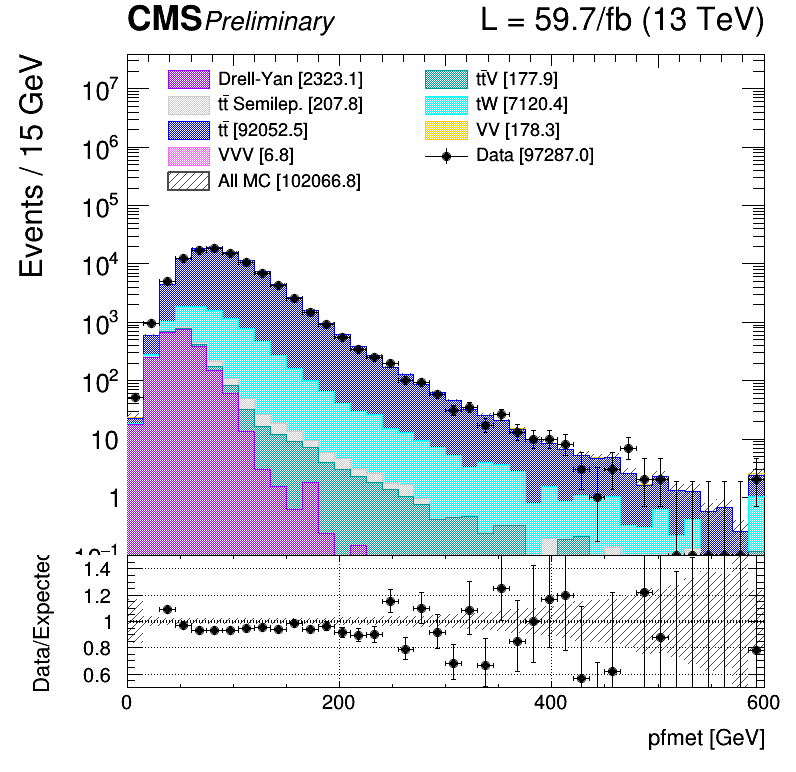
\includegraphics[width=1.0\textwidth, height=90pt]{figs/2018/log_cratio_ttbarCR_ll_METcorrected_pt.png}
    		\end{center}		
		\end{column}
\end{columns} \vfill
\end{frame}

\begin{frame}{DY Rin-out method}
\justifying
We want to \textbf{estimate the DY yields outside of the Z-peak from the data}:

\begin{itemize}
\justifying
\item Given the presence of large backgrounds (such as $t \bar t$) in the analysis region, we go inside of the Z-peak to compute the \alert{Rin-out factor}:
\begin{equation*}
N^{out}_{DY} = N^{in}_{DY, data} \cdot \kappa \cdot \left (\frac{N^{out}_{DY, MC}}{N^{in}_{DY, MC}} \right ) \equiv N^{in}_{DY, data} \cdot \frac{R_{out/in,\text{ } MC}^{0bj}}{R_{out/in,\text{ } data}^{0bj}} \cdot R_{out/in,\text{ } MC}
\end{equation*}
\item To avoid any bias, the contamination of non-peaking backgrounds is removed and we correct this factor by the ratio $\kappa$ between the data/MC transfer factors in a CR close to the SR (asking for 0 b-jet instead of 1);
\item We then get this Rin-out in \textbf{bins of MET and for each channel ($ee$, $\mu \mu$) separately}:
\end{itemize}

\begin{figure}[htbp]
\begin{center}
\begin{minipage}[b]{.32\textwidth}
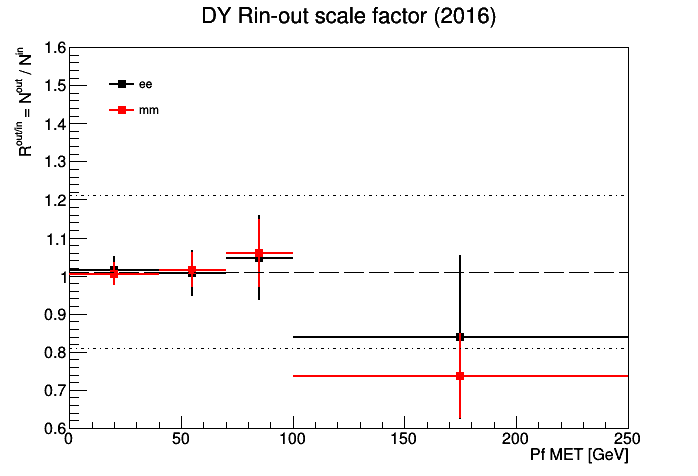
\includegraphics[width=4cm, height=3cm]{figs/Rinout2016.png}
\end{minipage} \hfill
\begin{minipage}[b]{.32\textwidth}
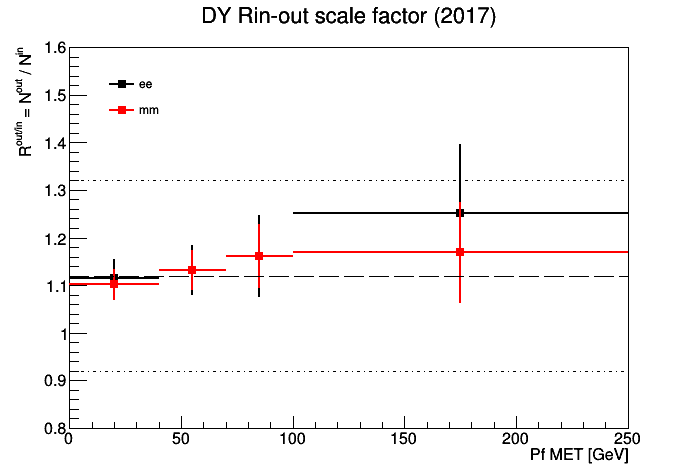
\includegraphics[width=4cm, height=3cm]{figs/Rinout2017.png}
\end{minipage} \hfill
\begin{minipage}[b]{.32\textwidth}
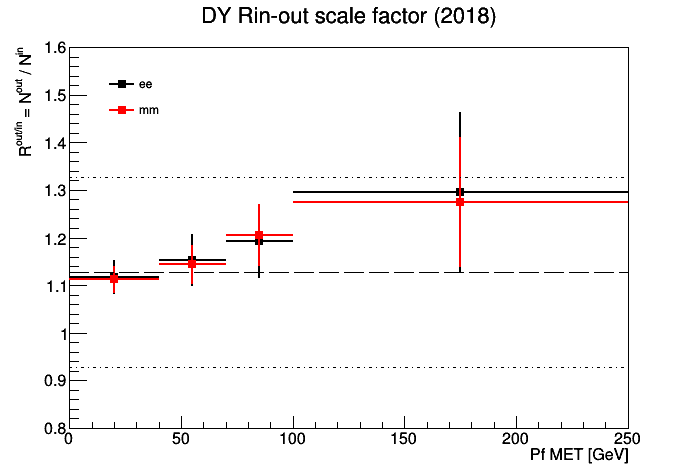
\includegraphics[width=4cm, height=3cm]{figs/Rinout2018.png}
\end{minipage} \hfill
\end{center}
\end{figure} \vfill

\vspace{-5pt}
A flat scale factor and a fixed 20\% systematic uncertainty is then applied to the DY. This method and the difference in statistics are still being studied. \vfill
\end{frame}

\begin{frame}{DY control region}
\justifying
\begin{columns}
\begin{column}{1.09\textwidth}
\begin{block}{\centering $ll$ channel}\end{block}
\end{column}
\end{columns} \vspace{-5pt}
\begin{columns}
		\begin{column}{0.33\textwidth}
			\begin{center}
			\vspace{-8pt}
			\begin{block}{\centering 2016}\end{block}\vspace{5pt}
     			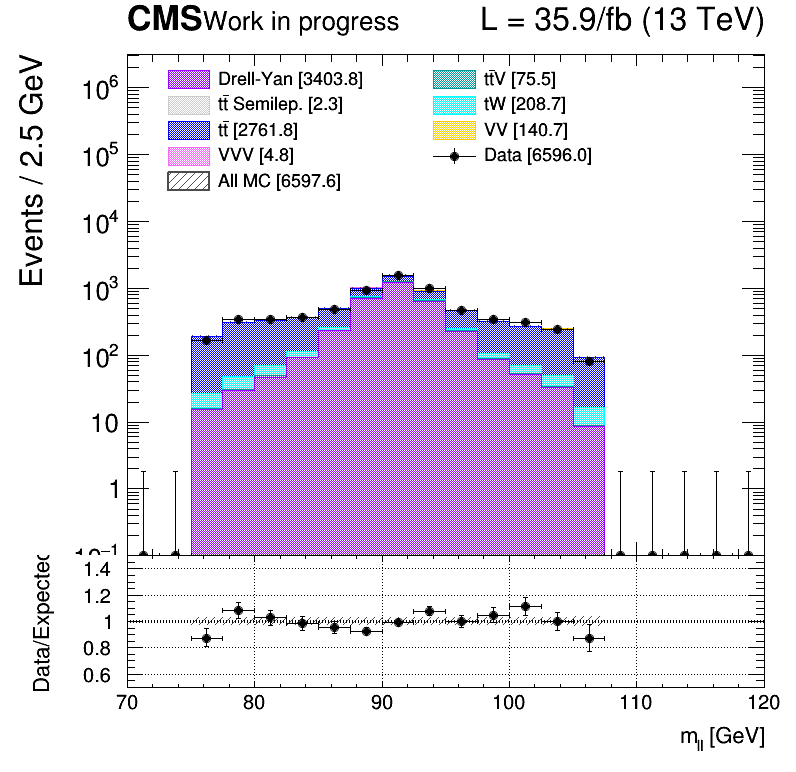
\includegraphics[width=1.0\textwidth, height=90pt]{figs/2016/log_cratio_dyCR_ll_mllpeak.png}
    		\end{center}		
		\end{column} 
		\begin{column}{0.33\textwidth}
			\begin{center}
			\vspace{-8pt}
			\begin{block}{\centering 2017}\end{block}\vspace{5pt}
     			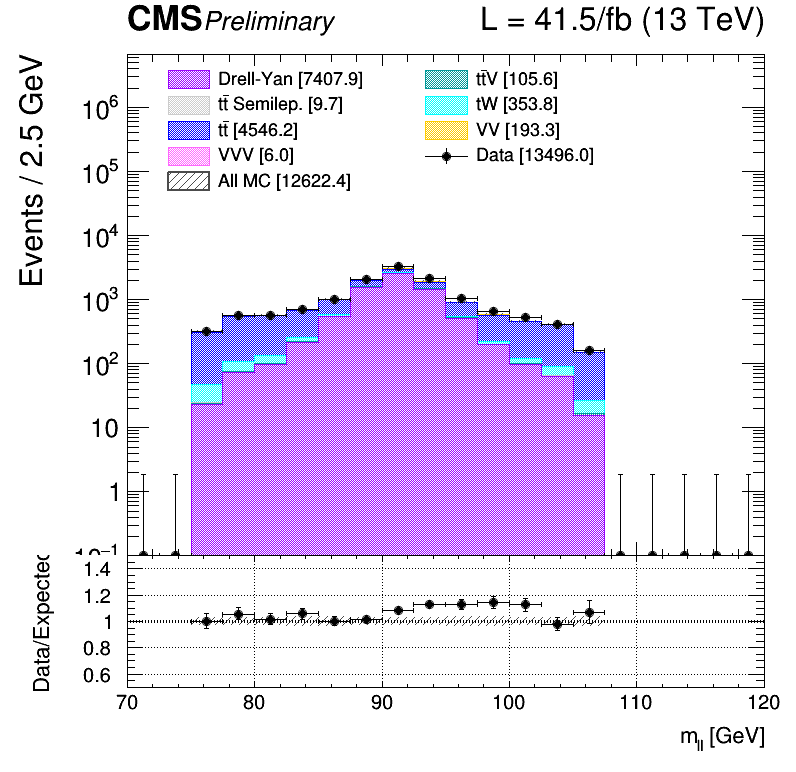
\includegraphics[width=1.0\textwidth, height=90pt]{figs/2017/log_cratio_dyCR_ll_mllpeak.png}
    		\end{center}		
		\end{column} 
		\begin{column}{0.33\textwidth}
			\begin{center}
			\vspace{-8pt}
			\begin{block}{\centering 2018}\end{block}\vspace{5pt}
     			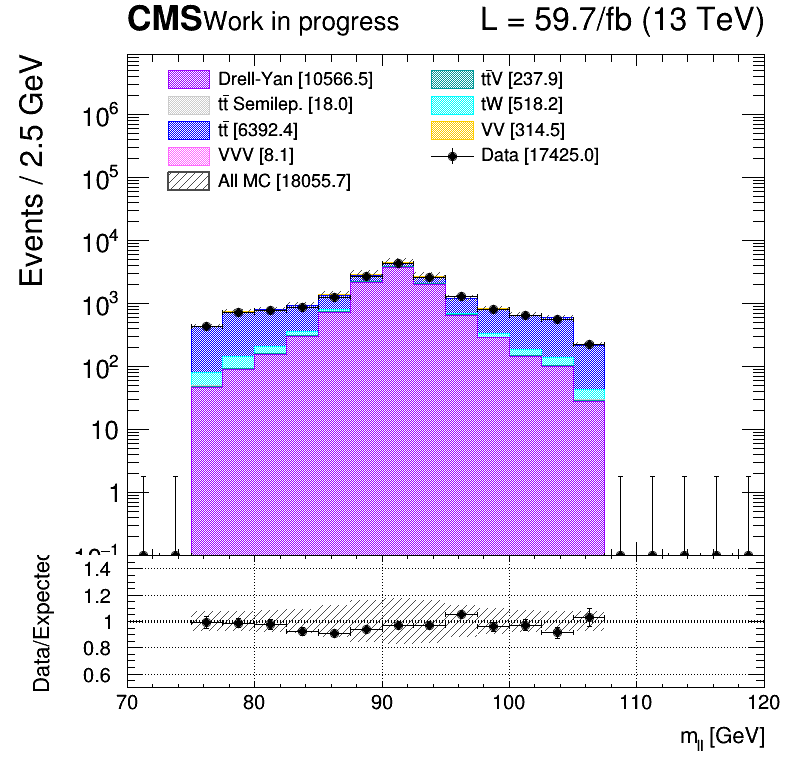
\includegraphics[width=1.0\textwidth, height=90pt]{figs/2018/log_cratio_dyCR_ll_mllpeak.png}
    		\end{center}		
		\end{column}
\end{columns}
\vspace{-10pt}
\begin{columns}
		\begin{column}{0.33\textwidth}
			\begin{center}
				%\begin{block}{\centering Puppi MET}\end{block}	
     			\includegraphics[width=1.0\textwidth, height=90pt]{figs/2016/log_cratio_dyCR_ll_METcorrected_pt.png}
    		\end{center}		
		\end{column}
		\begin{column}{0.33\textwidth}
			\begin{center}
				%\begin{block}{\centering njet}\end{block}	
     			\includegraphics[width=1.0\textwidth, height=90pt]{figs/2017/log_cratio_dyCR_ll_METcorrected_pt.png}
    		\end{center}		
		\end{column}
		\begin{column}{0.33\textwidth}
			\begin{center}
				%\begin{block}{\centering nbjet}\end{block}	
     			\includegraphics[width=1.0\textwidth, height=90pt]{figs/2018/log_cratio_dyCR_ll_METcorrected_pt.png}
    		\end{center}		
		\end{column}
\end{columns} \vfill

The 0-bjet correction allows us to fix the data/MC discrepancies observed. A large systematic uncertainty is associated to this background, minor in the signal regions. \vfill
\end{frame}

\begin{frame}{Non-prompt contamination I}
\justifying
Fake leptons detection (mostly jets misidentified or leptons coming from semileptonic b-quark decays $b \rightarrow cW \rightarrow c l \nu$) in the detector needs to be taken into account, through a \alert{data-driven tight-to-loose method} since the Monte-Carlo is not reliable in this case: \vfill

\begin{block}{\centering Fake rate}\end{block} \vspace{-5pt}
\begin{itemize}
\justifying
\item A QCD enriched region is defined with a looser particle selection criteria, where the misidentification should be high;
\item Any eventual contamination from electroweak processes in this region is removed;
\item The \alert{fake rate} is defined as the ratio between the fakeable object (lepton-like objects passing only the loose isolation requirements) and fully selected objects yields.
\end{itemize} \vfill

\begin{block}{\centering Prompt rate}\end{block} \vspace{-5pt}
\begin{itemize}
\justifying
\item The \alert{prompt rate}, taking into account the real lepton contamination is calculated in a Z enriched region from a general tag and probe method.
\end{itemize} \vfill

Then, we calculate from data an extrapolation factor to go back to the signal region of the analysis and the results obtained are checked in a \alert{same sign control region}. \vfill
\end{frame}

\begin{frame}{Non-prompt contamination II}
\justifying
\begin{block}{\centering 2016 fake rate}\end{block}
\vspace{-15pt}
\begin{figure}[htbp]
\begin{center}
\begin{minipage}[b]{.49\textwidth}
\begin{block}{\centering Electron}\end{block}
\begin{center}
\includegraphics[width=4.2cm, height=3.7cm]{figs/Ele_FR_pt_35GeV_2016.png}
\end{center}
\end{minipage} \hfill
\begin{minipage}[b]{.49\textwidth}
\begin{block}{\centering Muon}\end{block}
\begin{center}
\includegraphics[width=4.2cm, height=3.7cm]{figs/Muon_FR_pt_25GeV_2016.png}
\end{center}
\end{minipage} \hfill
\end{center}
\end{figure} \vfill

\vspace{-10pt}
\begin{block}{\centering 2016 prompt rate}\end{block} \vspace{-10pt}
\begin{figure}[htbp]
\begin{center}
\begin{minipage}[b]{.49\textwidth}
\begin{center}
\includegraphics[width=4.2cm, height=3.7cm]{figs/Ele_PR_pt_2016.png}
\end{center}
\end{minipage} \hfill
\begin{minipage}[b]{.49\textwidth}
\begin{center}
\includegraphics[width=4.2cm, height=3.7cm]{figs/Muon_PR_pt_2016.png}
\end{center}
\end{minipage} \hfill
\end{center}
\end{figure} \vfill

A \textbf{flat 30\% systematic uncertainty} is finally associated to this background in order to cover the statistical uncertainty plus eventual discrepancies in this control region. \vfill
\end{frame}

\begin{frame}{Same sign control region}
\justifying
This is checked in a dedicated same sign control region. \vfill
\begin{columns}
\begin{column}{1.09\textwidth}
\begin{block}{\centering $ll$ channel}\end{block}
\end{column}
\end{columns} \vspace{-5pt}
\begin{columns}
		\begin{column}{0.33\textwidth}
			\begin{center}
			\vspace{-8pt}
			\begin{block}{\centering 2016}\end{block}\vspace{10pt}
     			\includegraphics[width=1.0\textwidth, height=90pt]{figs/2016/log_cratio_SSCR_ll_mll.png}
    		\end{center}		
		\end{column} 
		\begin{column}{0.33\textwidth}
			\begin{center}
			\vspace{-8pt}
			\begin{block}{\centering 2017}\end{block}\vspace{10pt}
     			\includegraphics[width=1.0\textwidth, height=90pt]{figs/2017/log_cratio_SSCR_ll_mll.png}
    		\end{center}		
		\end{column} 
		\begin{column}{0.33\textwidth}
			\begin{center}
			\vspace{-8pt}
			\begin{block}{\centering 2018}\end{block}\vspace{10pt}
     			\includegraphics[width=1.0\textwidth, height=90pt]{figs/2018/log_cratio_SSCR_ll_mll.png}
    		\end{center}		
		\end{column}
\end{columns}  \vspace{-5pt}
\begin{columns}
		\begin{column}{0.33\textwidth}
			\begin{center}
				%\begin{block}{\centering Puppi MET}\end{block}	
     			\includegraphics[width=1.0\textwidth, height=90pt]{figs/2016/log_cratio_SSCR_ll_METcorrected_pt.png}
    		\end{center}		
		\end{column}
		\begin{column}{0.33\textwidth}
			\begin{center}
				%\begin{block}{\centering njet}\end{block}	
     			\includegraphics[width=1.0\textwidth, height=90pt]{figs/2017/log_cratio_SSCR_ll_METcorrected_pt.png}
    		\end{center}		
		\end{column}
		\begin{column}{0.33\textwidth}
			\begin{center}
				%\begin{block}{\centering nbjet}\end{block}	
     			\includegraphics[width=1.0\textwidth, height=90pt]{figs/2018/log_cratio_SSCR_ll_METcorrected_pt.png}
    		\end{center}		
		\end{column}
\end{columns} \vfill
\end{frame}

\begin{frame}{$ttV$ prediction}
\justifying
This process is taken directly from MC, and crosschecked in a dedicated control region. \vfill
\begin{columns}
\begin{column}{1.09\textwidth}
\begin{block}{\centering $ll$ channel}\end{block}
\end{column}
\end{columns} \vspace{-5pt}
\begin{columns}
		\begin{column}{0.33\textwidth}
			\begin{center}
			\vspace{-8pt}
			\begin{block}{\centering 2016}\end{block}\vspace{10pt}
     			\includegraphics[width=1.0\textwidth, height=90pt]{figs/2016/log_cratio_ttVCR_ll_mll.png}
    		\end{center}		
		\end{column} 
		\begin{column}{0.33\textwidth}
			\begin{center}
			\vspace{-8pt}
			\begin{block}{\centering 2017}\end{block}\vspace{10pt}
     			\includegraphics[width=1.0\textwidth, height=90pt]{figs/2017/log_cratio_ttVCR_ll_mll.png}
    		\end{center}		
		\end{column} 
		\begin{column}{0.33\textwidth}
			\begin{center}
			\vspace{-8pt}
			\begin{block}{\centering 2018}\end{block}\vspace{10pt}
     			\includegraphics[width=1.0\textwidth, height=90pt]{figs/2018/log_cratio_ttVCR_ll_mll.png}
    		\end{center}		
		\end{column}
\end{columns} \vspace{-5pt}
\begin{columns}
		\begin{column}{0.33\textwidth}
			\begin{center}
				%\begin{block}{\centering Puppi MET}\end{block}	
     			\includegraphics[width=1.0\textwidth, height=90pt]{figs/2016/log_cratio_ttVCR_ll_METcorrected_pt.png}
    		\end{center}		
		\end{column}
		\begin{column}{0.33\textwidth}
			\begin{center}
				%\begin{block}{\centering njet}\end{block}	
     			\includegraphics[width=1.0\textwidth, height=90pt]{figs/2017/log_cratio_ttVCR_ll_METcorrected_pt.png}
    		\end{center}		
		\end{column}
		\begin{column}{0.33\textwidth}
			\begin{center}
				%\begin{block}{\centering nbjet}\end{block}	
     			\includegraphics[width=1.0\textwidth, height=90pt]{figs/2018/log_cratio_ttVCR_ll_METcorrected_pt.png}
    		\end{center}		
		\end{column}
\end{columns} \vfill
\end{frame}


















\begin{frame}[standout]
Systematic uncertainties
\end{frame}

\begin{frame}{Systematic uncertainties}
\justifying
Most of the systematics to be considered (on top of the statistical uncertainties) are already in place, such as: \vfill

\begin{block}{\centering Theoretical uncertainties}\end{block} 

\begin{itemize}
\justifying
\item PDF and higher order corrections, underlying event and parton shower, renormalization and factorization scales.
\end{itemize} \vfill

\begin{block}{\centering Experimental uncertainties}\end{block}

\begin{itemize}
\justifying
\item Luminosity, pileup modeling, lepton trigger, lepton efficiency and energy scale, jet energy scale, MET mismodelling, b-tagging efficiency, top $p_T$ reweighting.
\end{itemize} \vfill

\begin{block}{\centering Background specific uncertainties}\end{block}

\begin{itemize}
\justifying
\item Drell-Yan and non-prompt backgrounds related uncertainties.
\end{itemize} \vfill

\alert{Disclaimer}: this part of the analysis still needs to be checked/optimized, so results shown next are preliminary and expected to change in the future. \vfill
\end{frame}

\begin{frame}[standout]
Results obtained
\end{frame}

\begin{frame}{Upper limits without systematics}
\begin{columns}
\begin{column}{1.09\textwidth}
\begin{block}{\centering Scalar upper limits}\end{block}
\end{column}
\end{columns} \vspace{-5pt}
\begin{columns}
		\begin{column}{0.33\textwidth}
			\begin{center}
			\vspace{-8pt}
			\begin{block}{\centering 2016}\end{block} \vspace{-10pt}
     			\includegraphics[width=1.0\textwidth, height=90pt]{figs/limit_scalar2016.png}
    		\end{center}		
		\end{column} 
		\begin{column}{0.33\textwidth}
			\begin{center}
			\vspace{-8pt}
			\begin{block}{\centering 2017}\end{block} \vspace{-10pt}
     			\includegraphics[width=1.0\textwidth, height=90pt]{figs/limit_scalar2017.png}
    		\end{center}		
		\end{column} 
		\begin{column}{0.33\textwidth}
			\begin{center}
			\vspace{-8pt}
			\begin{block}{\centering 2018}\end{block} \vspace{-10pt}
     			\includegraphics[width=1.0\textwidth, height=90pt]{figs/limit_scalar2018.png}
    		\end{center}		
		\end{column}
\end{columns}

\begin{columns}
\begin{column}{1.09\textwidth}
\begin{block}{\centering Pseudoscalar upper limits}\end{block}
\end{column}
\end{columns} \vspace{-15pt}
\begin{columns}
		\begin{column}{0.33\textwidth}
			\begin{center}
				%\begin{block}{\centering Puppi MET}\end{block}	
     			\includegraphics[width=1.0\textwidth, height=90pt]{figs/limit_pseudo2016.png}
    		\end{center}		
		\end{column}
		\begin{column}{0.33\textwidth}
			\begin{center}
				%\begin{block}{\centering njet}\end{block}	
     			\includegraphics[width=1.0\textwidth, height=90pt]{figs/limit_pseudo2017.png}
    		\end{center}		
		\end{column}
		\begin{column}{0.33\textwidth}
			\begin{center}
				%\begin{block}{\centering nbjet}\end{block}	
     			\includegraphics[width=1.0\textwidth, height=90pt]{figs/limit_pseudo2018.png}
    		\end{center}		
		\end{column}
\end{columns} \vfill
\end{frame}

\begin{frame}{Run II legacy limits}
\justifying
\textbf{Disclaimer:} preliminary comparison done with some systematics missing, so results are expected to change a bit. \vfill

\begin{columns}
	\begin{column}{0.5 \textwidth}
\begin{center}
\begin{block}{\centering Scalar mediators}\end{block} \vspace{-10pt}
\includegraphics[width=5.4cm, height=4.8cm]{figs/limit_scalar_allYears.png}
\end{center}
\end{column}
	\begin{column}{0.5 \textwidth}
\begin{figure}[htbp]
\begin{center}
\begin{block}{\centering Pseudoscalar mediators}\end{block} \vspace{-8pt}
\includegraphics[width=5.4cm, height=4.8cm]{figs/limit_pseudo_allYears.png}
\end{center}
\end{figure}
	\end{column}
	\end{columns} \vfill
\end{frame}

\begin{frame}{Conclusions}
\justifying
A search for \alert{dark matter produced in association with either one or two top quarks} is on-going using the Latino framework:

\begin{itemize}
\justifying
\item This search is considering the \textbf{Run II legacy dataset} collected by the CMS detector;
\item At IFCA, our efforts are entirely focused on the \textbf{dilepton final state};
\item This search is performed by defining a ANN, training it to be able to recognize background and signal events, to separate them and \textbf{increase the signal efficiency};
\item First time that such a combination will be performed considering this canal, which should increase by a lot the limits published in 2016; 
\item We expect this analysis \alert{to be approved by June}.
\end{itemize} \vfill

In general, using the Latino framework was extremely helpful given its reliability and global ease of use. \vfill
\end{frame}


\backupbegin

\begin{frame}[standout]
Back up
\end{frame}

\begin{frame}{CMS relevant results I}
\justifying
CMS dilepton channel 2016 results published: \vfill

\begin{figure}[htbp]
\centering
\begin{minipage}[b]{.5\textwidth}
\includegraphics[width=5.3cm, height=4.9cm]{figs/Juan_scalar_limits.png}
\end{minipage}\hfill
\begin{minipage}[b]{.5\textwidth}
\includegraphics[width=5.3cm, height=4.9cm]{figs/Juan_pseudo_limits.png}
\end{minipage}\hfill
\end{figure} \vfill
\end{frame}

\begin{frame}{CMS relevant results II}
\justifying
\vspace{5pt}
A \textbf{combination} of both the $t/ \bar t$+DM and $t \bar t$+DM processes has also been performed. \vfill
The inclusion of the single top signal process \alert{improved up to a factor 2} the limits obtained by the $t \bar t$ analysis on its own. This analysis: %\cite{PreviousSingleDoubleTopAllLep13CMS}. 

\begin{itemize}
\item Only considered the 2016 data-taking period;
\item And only considered the semi-leptonic and hadronic final states.
\end{itemize} \vfill

\begin{center}
\begin{columns}
	\begin{column}{1.0\textwidth}
		\begin{center}
			%\begin{block}{\centering $t \bar t$+DM limits}\end{block}				
			%\alert{\textbf{$t \bar t$ + DM model}} \\ \vspace{5pt}
			\includegraphics[width=1.0\textwidth]{figs/limitsprevious.png}
    		 \end{center}
	\end{column} \hfill
\end{columns}
\end{center} \vfill

Scalar (pseudoscalar) mediators were with this combination \alert{excluded up to 290 (300) GeV} at the 95\% confidence level. \vfill %The inclusion of the full Run II dataset and the dilepton final state \textbf{is expected to improve these results}.
\end{frame}

\begin{frame}{ATLAS relevant results I}
\justifying
ATLAS dilepton channel Run II legacy resuts from ICHEP 2020: \vfill

 \begin{figure}[htbp]
\centering
\includegraphics[width=10.5cm, height=4.7cm]{figs/ATLASICHEP.png}
\end{figure} \vfill
\end{frame}

\begin{frame}{ATLAS relevant results II}
\justifying
The ATLAS collaboration does not perform any combination between the different channels though. \vfill

\begin{figure}[htbp]
\centering
\begin{minipage}[b]{.5\textwidth}
\includegraphics[width=5.3cm, height=4cm]{figs/ATLASttDM_scalar.png}
\end{minipage}\hfill
\begin{minipage}[b]{.5\textwidth}
\includegraphics[width=5.3cm, height=4cm]{figs/ATLASttDM_pseudoscalar.png}
\end{minipage}\hfill
\end{figure} \vfill
\end{frame}

\begin{frame}{2016 data samples}
\justifying
\begin{table}
\begin{center}
\resizebox{0.65\textwidth}{!}{
\begin{tabular}{ c|c|c } 
 \hline
 Dataset & Events (size) & $\mathcal{L}$ [fb$^{-1}$] \\
\hline
\textbf{Run 2016B} & & \\
/DoubleEG/Run2016B\_ver2-Nano02Apr2020\_ver2-v1/NANOAOD & 143073268 (99.4Gb) & \multirow{ 5}{*}{5.8}  \\
/DoubleMuon/Run2016B\_ver2-Nano02Apr2020\_ver2-v1/NANOAOD & 82535526 (53.2Gb) &   \\
 /MuonEG/Run2016B\_ver2-Nano02Apr2020\_ver2-v1/NANOAOD & 32727796 (26.8Gb) & \\
 /SingleElectron/Run2016B\_ver2-Nano02Apr2020\_ver2-v1/NANOAOD & 246440440 (167.8Gb) & \\
 /SingleMuon/Run2016B\_ver2-Nano02Apr2020\_ver2-v1/NANOAOD & 158145722 (96.4Gb) & \\
 \hline
 \textbf{Run 2016C} & & \\
 /DoubleEG/Run2016C-Nano02Apr2020-v1/NANOAOD & 47677856 (35.3Gb) & \multirow{ 5}{*}{2.6} \\
 /DoubleMuon/Run2016C-Nano02Apr2020-v1/NANOAOD & 27934629 (19.7Gb) & \\
 /MuonEG/Run2016C-Nano02Apr2020-v1/NANOAOD & 15405678 (12.8Gb) & \\
 /SingleElectron/Run2016C-Nano02Apr2020-v1/NANOAOD & 97259854 (69.3Gb) & \\
 /SingleMuon/Run2016C-Nano02Apr2020-v1/NANOAOD & 67441308 (42.4Gb) & \\
 \hline
 \textbf{Run 2016D} & & \\
 /DoubleEG/Run2016D-Nano02Apr2020-v1/NANOAOD & 53324960 (39.6Gb) & \multirow{ 5}{*}{4.2} \\
 /DoubleMuon/Run2016D-Nano02Apr2020-v1/NANOAOD & 33861745 (24.1Gb) & \\
 /MuonEG/Run2016D-Nano02Apr2020-v1/NANOAOD & 23482352 (19.4Gb) & \\
 /SingleElectron/Run2016D-Nano02Apr2020-v1/NANOAOD & 148167727 (104.4Gb) & \\
 /SingleMuon/Run2016D-Nano02Apr2020-v1/NANOAOD & 98017996 (61.3Gb) & \\
 \hline
 \textbf{Run 2016E} & & \\
 /DoubleEG/Run2016E-Nano02Apr2020-v1/NANOAOD & 49877710 (37.9Gb) & \multirow{ 5}{*}{4.0} \\
 /DoubleMuon/Run2016E-Nano02Apr2020-v1/NANOAOD & 28246946 (20.8Gb) & \\
 /MuonEG/Run2016E-Nano02Apr2020-v2/NANOAOD & 22519303 (19.0Gb) & \\
 /SingleElectron/Run2016E-Nano02Apr2020-v1/NANOAOD & 117321545 (86.5Gb) & \\
 /SingleMuon/Run2016E-Nano02Apr2020-v1/NANOAOD & 90984718 (58.7Gb) & \\
 \hline
 \textbf{Run 2016F} & & \\
 /DoubleEG/Run2016F-Nano02Apr2020-v1/NANOAOD & 34577629 (26.9Gb) & \multirow{ 5}{*}{3.1} \\
 /DoubleMuon/Run2016F-Nano02Apr2020-v1/NANOAOD & 20329921 (15.3Gb) & \\
 /MuonEG/Run2016F-Nano02Apr2020-v1/NANOAOD & 16002165 (13.6Gb) & \\
 /SingleElectron/Run2016F-Nano02Apr2020-v1/NANOAOD & 70593532 (51.4Gb) & \\
 /SingleMuon/Run2016F-Nano02Apr2020-v1/NANOAOD & 65489554 (42.4Gb) & \\
 \hline
 \textbf{Run 2016G} & & \\
 /DoubleEG/Run2016G-Nano02Apr2020-v1/NANOAOD & 78797031 (61.6Gb) & \multirow{ 5}{*}{7.6} \\
 /DoubleMuon/Run2016G-Nano02Apr2020-v1/NANOAOD & 45235604 (34.2Gb) & \\
 /MuonEG/Run2016G-Nano02Apr2020-v1/NANOAOD & 33854612 (29.0Gb) & \\
 /SingleElectron/Run2016G-Nano02Apr2020-v1/NANOAOD & 153363109 (109.2Gb) & \\
 /SingleMuon/Run2016G-Nano02Apr2020-v1/NANOAOD & 149912248 (94.6Gb) & \\
 \hline
 \textbf{Run 2016H} & & \\
 /DoubleEG/Run2016H-Nano02Apr2020-v1/NANOAOD & 85388734 (67.7Gb) & \multirow{ 5}{*}{8.6} \\
 /DoubleMuon/Run2016H-Nano02Apr2020-v1/NANOAOD & 48912812 (37.3Gb) & \\
 /MuonEG/Run2016H-Nano02Apr2020-v1/NANOAOD & 29236516 (26.0Gb) & \\
 /SingleElectron/Run2016H-Nano02Apr2020-v1/NANOAOD & 128854598 (93.8Gb) & \\
 /SingleMuon/Run2016H-Nano02Apr2020-v1/NANOAOD & 174035164 (110.2Gb) & \\
 \hline
\end{tabular}
}
\end{center}
\end{table}
\end{frame}

\begin{frame}{2017 data samples}
\justifying
\begin{table}
\begin{center}
\resizebox{0.8\textwidth}{!}{
\begin{tabular}{ c|c|c } 
 \hline
 Dataset & Events (size) & $\mathcal{L}$ [fb$^{-1}$] \\
\hline
\textbf{Run 2017B} & & \\
/DoubleEG/Run2017B-Nano02Apr2020-v1/NANOAOD & 58088760 (46.6Gb) & \multirow{ 5}{*}{4.8} \\
/DoubleMuon/Run2017B-Nano02Apr2020-v1/NANOAOD & 14501767 (10.8Gb) & \\
/SingleElectron/Run2017B-Nano02Apr2020-v1/NANOAOD & 60537490 (42.2Gb) & \\
/SingleMuon/Run2017B-Nano02Apr2020-v1/NANOAOD & 136300266 (86.2Gb) & \\
/MuonEG/Run2017B-Nano02Apr2020-v1/NANOAOD & 4453465 (4.1Gb) & \\
 \hline
 \textbf{Run 2017C} & & \\
 /DoubleEG/Run2017C-Nano02Apr2020-v1/NANOAOD & 65181125 (53.8Gb) & \multirow{ 5}{*}{9.7} \\
 /DoubleMuon/Run2017C-Nano02Apr2020-v1/NANOAOD & 49636525 (39.5Gb) & \\
 /SingleElectron/Run2017C-Nano02Apr2020-v1/NANOAOD & 136637888 (102.5Gb) & \\
 /SingleMuon/Run2017C-Nano02Apr2020-v1/NANOAOD & 165652756 (109.5Gb) & \\
 /MuonEG/Run2017C-Nano02Apr2020-v1/NANOAOD & 15595214 (15.0Gb) & \\
 \hline
 \textbf{Run 2017D} & & \\
/DoubleEG/Run2017D-Nano02Apr2020-v1/NANOAOD & 25911432 (21.6Gb) & \multirow{ 5}{*}{4.2} \\
/DoubleMuon/Run2017D-Nano02Apr2020-v1/NANOAOD & 23075733 (18.6Gb) & \\
/SingleElectron/Run2017D-Nano02Apr2020-v1/NANOAOD & 51526710 (38.5Gb) & \\
/SingleMuon/Run2017D-Nano02Apr2020-v1/NANOAOD & 70361660 (47.2Gb) & \\
 /MuonEG/Run2017D-Nano02Apr2020-v1/NANOAOD & 9164365 (8.9Gb) & \\
 \hline
 \textbf{Run 2017E} & & \\
/DoubleEG/Run2017E-Nano02Apr2020-v1/NANOAOD & 56233597 (49.8Gb) & \multirow{ 5}{*}{9.3} \\
/DoubleMuon/Run2017E-Nano02Apr2020-v1/NANOAOD & 51589091 (44.4Gb) & \\
/SingleElectron/Run2017E-Nano02Apr2020-v1/NANOAOD & 102121689 (81.3Gb) & \\
/SingleMuon/Run2017E-Nano02Apr2020-v1/NANOAOD & 154630534 (111.0Gb) & \\
/MuonEG/Run2017E-Nano02Apr2020-v1/NANOAOD & 19043421 (19.2Gb) & \\
 \hline
\textbf{Run 2017F} & & \\ 
/DoubleEG/Run2017F-Nano02Apr2020-v1/NANOAOD & 74307066 (67.1Gb) & \multirow{ 5}{*}{13.5} \\
/DoubleMuon/Run2017F-Nano02Apr2020-v1/NANOAOD & 79756560 (68.0Gb) & \\
/SingleElectron/Run2017F-Nano02Apr2020-v1/NANOAOD & 128467223 (105.2Gb) & \\
/SingleMuon/Run2017F-Nano02Apr2020-v1/NANOAOD & 242135500 (178.3Gb) \\
 /MuonEG/Run2017F-Nano02Apr2020-v1/NANOAOD & 25776363 (26.3Gb) & \\
 \hline
\end{tabular}
}
\end{center}
\end{table}
\end{frame}

\begin{frame}{2018 data samples}
\justifying
\begin{table}
\begin{center}
\resizebox{0.8\textwidth}{!}{
\begin{tabular}{ c|c|c } 
 \hline
 Dataset & Events (size) & $\mathcal{L}$ [fb$^{-1}$] \\
\hline
\textbf{Run 2018A} & & \\
 /DoubleMuon/Run2018A-Nano02Apr2020-v1/NANOAOD & 75499908 (62.6Gb) & \multirow{ 4}{*}{13.5} \\
 /EGamma/Run2018A-Nano02Apr2020-v1/NANOAOD & 327843843 (261.8Gb) & \\
 /SingleMuon/Run2018A-Nano02Apr2020-v1/NANOAOD & 241608232 (167.7Gb) & \\
 /MuonEG/Run2018A-Nano02Apr2020-v1/NANOAOD & 32958503 (32.3Gb) & \\
 \hline
\textbf{Run 2018B} & & \\
 /DoubleMuon/Run2018B-Nano02Apr2020-v1/NANOAOD & 35057758 (28.3Gb) & \multirow{ 4}{*}{6.8} \\
 /EGamma/Run2018B-Nano02Apr2020-v1/NANOAOD & 153822427 (123.1Gb) & \\
 /SingleMuon/Run2018B-Nano02Apr2020-v1/NANOAOD & 119918017 (82.3Gb) & \\
 /MuonEG/Run2018B-Nano02Apr2020-v1/NANOAOD & 16211567 (15.8Gb) & \\
 \hline
 \textbf{Run 2018C} & & \\
/DoubleMuon/Run2018C-Nano02Apr2020-v1/NANOAOD & 34565869 (27.6Gb) & \multirow{ 4}{*}{6.6} \\
/EGamma/Run2018C-Nano02Apr2020-v1/NANOAOD & 147827904 (119.2Gb) & \\
/SingleMuon/Run2018C-Nano02Apr2020-v1/NANOAOD & 110032072 (75.7Gb) & \\
/MuonEG/Run2018C-Nano02Apr2020-v1/NANOAOD & 15652198 (15.3Gb) & \\
 \hline
 \textbf{Run 2018D} & & \\
/DoubleMuon/Run2018D-Nano02Apr2020\_ver2-v1/NANOAOD & 168605834 (128.6Gb) & \multirow{ 4}{*}{32.0} \\
/EGamma/Run2018D-Nano02Apr2020-v1/NANOAOD & 751348648 (583.6Gb) & \\
/SingleMuon/Run2018D-Nano02Apr2020-v1/NANOAOD & 513867253 (344.5Gb) & \\
/MuonEG/Run2018D-Nano02Apr2020\_ver2-v1/NANOAOD & 71961587 (68.6Gb) & \\
 \hline
\end{tabular}
}
\end{center}
\end{table}
\end{frame}

\begin{frame}{2016 MC samples}
\justifying
\begin{table}
\begin{center}
\resizebox{0.8\textwidth}{!}{
\begin{tabular}{ c|c|c } 
 \hline
 Process & Sample & Cross section [pb] \\
\hline
\multirow{1}{*}{Drell-Yan} & DYJetsToLL\_M-10to50\_TuneCUETP8M1\_13TeV-madgraphMLM-pythia8 ($H_T < 70$ GeV) & 18610.0 \\
& DYJetsToLL\_M-5to50\_HT-70to100\_TuneCUETP8M1\_13TeV-madgraphMLM-pythia8 & 303.8 \\
& DYJetsToLL\_M-5to50\_HT-100to200\_TuneCUETP8M1\_13TeV-madgraphMLM-pythia8 & 224.2 \\
& DYJetsToLL\_M-5to50\_HT-200to400\_TuneCUETP8M1\_13TeV-madgraphMLM-pythia8 & 37.2 \\
& DYJetsToLL\_M-5to50\_HT-400to600\_TuneCUETP8M1\_13TeV-madgraphMLM-pythia8 & 3.581 \\
& DYJetsToLL\_M-5to50\_HT-600toInf\_TuneCUETP8M1\_13TeV-madgraphMLM-pythia8 & 1.124 \\
& DYJetsToLL\_M-50\_TuneCUETP8M1\_13TeV-madgraphMLM-pythia8 ($H_T < 70$ GeV) & 6025.20 \\
& DYJetsToLL\_M-50\_HT-70to100\_TuneCUETP8M1\_13TeV-madgraphMLM-pythia8 & 169.9 \\
& DYJetsToLL\_M-50\_HT-100to200\_TuneCUETP8M1\_13TeV-madgraphMLM-pythia8 & 147.4 \\
& DYJetsToLL\_M-50\_HT-200to400\_TuneCUETP8M1\_13TeV-madgraphMLM-pythia8 & 40.99 \\
& DYJetsToLL\_M-50\_HT-400to600\_TuneCUETP8M1\_13TeV-madgraphMLM-pythia8 & 5.678 \\
& DYJetsToLL\_M-50\_HT-600to800\_TuneCUETP8M1\_13TeV-madgraphMLM-pythia8 & 1.367 \\
& DYJetsToLL\_M-50\_HT-800to1200\_TuneCUETP8M1\_13TeV-madgraphMLM-pythia8 & 0.6304 \\
& DYJetsToLL\_M-50\_HT-1200to2500\_TuneCUETP8M1\_13TeV-madgraphMLM-pythia8 & 0.1514 \\
& DYJetsToLL\_M-50\_HT-2500toInf\_TuneCUETP8M1\_13TeV-madgraphMLM-pythia8 & 0.003565 \\
\hline
\multirow{1}{*}{TTTo2L2Nu} & TTTo2L2Nu\_TuneCUETP8M2\_ttHtranche3\_13TeV-powheg-pythia8 & 87.310 \\
\hline
\multirow{1}{*}{Single top} & ST\_s-channel\_4f\_leptonDecays\_13TeV-amcatnlo-pythia8\_TuneCUETP8M1 & 3.360 \\
& ST\_t-channel\_antitop\_4f\_inclusiveDecays\_13TeV-powhegV2-madspin-pythia8\_TuneCUETP8M1 & 80.95 \\
& ST\_t-channel\_top\_4f\_inclusiveDecays\_13TeV-powhegV2-madspin-pythia8\_TuneCUETP8M1 & 136.02 \\
& ST\_tW\_antitop\_5f\_inclusiveDecays\_13TeV-powheg-pythia8\_TuneCUETP8M1 & 35.60 \\
& ST\_tW\_top\_5f\_inclusiveDecays\_13TeV-powheg-pythia8\_TuneCUETP8M1 & 35.60 \\
\hline
\multirow{1}{*}{ttV} & TTWJetsToLNu\_TuneCUETP8M1\_13TeV-amcatnloFXFX-madspin-pythia8 & 0.2043 \\
& ttZJets\_13TeV\_madgraphMLM-pythia8 & 0.7826 \\
& TTZToLLNuNu\_M-10\_TuneCUETP8M1\_13TeV-amcatnlo-pythia8 & 0.2529 \\
\hline
WW & WWTo2L2Nu\_13TeV-powheg & 12.178 \\
& WWJJToLNuLNu\_EWK\_noTop\_13TeV-madgraph-pythia8 & 0.34520 \\
& GluGluWWTo2L2Nu\_MCFM\_13TeV & 0.5905 \\
\hline
V$\gamma$/V$\gamma$* & WGToLNuG\_TuneCUETP8M1\_13TeV-madgraphMLM-pythia8 & 405.271 \\ 
& ZGTo2LG\_TuneCUETP8M1\_13TeV-amcatnloFXFX-pythia8 & 131.300 \\
& WZTo3LNu\_mllmin01\_13TeV-powheg-pythia8 & 58.59 \\
\hline
VZ & ZZTo2L2Nu\_13TeV\_powheg\_pythia8 & 0.5640 \\
& ZZTo2L2Q\_13TeV\_powheg\_pythia8 & 3.22 \\
& ZZTo4L\_TuneCP5\_13TeV\_powheg\_pythia8 & 1.212 \\
& WZTo2L2Q\_13TeV\_amcatnloFXFX\_madspin\_pythia8 & 5.595 \\
 \hline
 VVV & ZZZ\_TuneCUETP8M1\_13TeV-amcatnlo-pythia8 & 0.01398 \\
 & WZZ\_TuneCUETP8M1\_13TeV-amcatnlo-pythia8 & 0.05565 \\
 & WWZ\_TuneCUETP8M1\_13TeV-amcatnlo-pythia8 & 0.16510 \\
 & WWW\_4F\_TuneCUETP8M1\_13TeV-amcatnlo-pythia8 & 0.18331 \\
 \hline
 Non-Prompt & Data-driven (tight-to-loose method) & \\
 \hline
\end{tabular}
}
\end{center}
\end{table}
\end{frame}

\begin{frame}{2017 MC samples}
\justifying
\begin{table}
\begin{center}
\resizebox{0.8\textwidth}{!}{
\begin{tabular}{ c|c|c } 
 \hline
 Process & Sample & Cross section [pb] \\
\hline
\multirow{1}{*}{Drell-Yan} & DYJetsToLL\_M-10to50\_TuneCP5\_13TeV-madgraphMLM-pythia8 ($H_T < 100$ GeV) & 18610 \\
& DYJetsToLL\_M-4to50\_HT-100to200\_TuneCP5\_13TeV-madgraphMLM-pythia8 & 204.0 \\
& DYJetsToLL\_M-4to50\_HT-200to400\_TuneCP5\_13TeV-madgraphMLM-pythia8 & 54.39 \\
& DYJetsToLL\_M-4to50\_HT-400to600\_TuneCP5\_13TeV-madgraphMLM-pythia8 & 5.697 \\
& DYJetsToLL\_M-4to50\_HT-600toInf\_TuneCP5\_13TeV-madgraphMLM-pythia8 & 1.85 \\
& DYJetsToLL\_M-50\_TuneCP5\_13TeV-madgraphMLM-pythia8 ($H_T < 70$ GeV) & 6189.39 \\
& DYJetsToLL\_M-50\_HT-70to100\_TuneCP5\_13TeV-madgraphMLM-pythia8 & 169.9 \\
& DYJetsToLL\_M-50\_HT-100to200\_TuneCP5\_13TeV-madgraphMLM-pythia8 & 161.1 \\
& DYJetsToLL\_M-50\_HT-200to400\_TuneCP5\_13TeV-madgraphMLM-pythia8 & 48.66 \\
& DYJetsToLL\_M-50\_HT-400to600\_TuneCP5\_13TeV-madgraphMLM-pythia8 & 6.968 \\
& DYJetsToLL\_M-50\_HT-600to800\_TuneCP5\_13TeV-madgraphMLM-pythia8 & 1.743 \\
& DYJetsToLL\_M-50\_HT-800to1200\_TuneCP5\_13TeV-madgraphMLM-pythia8 & 0.8052 \\
& DYJetsToLL\_M-50\_HT-1200to2500\_TuneCP5\_13TeV-madgraphMLM-pythia8 & 0.1933 \\
& DYJetsToLL\_M-50\_HT-2500toInf\_TuneCP5\_13TeV-madgraphMLM-pythia8 & 0.003468 \\
\hline
\multirow{1}{*}{TTTo2L2Nu} & TTTo2L2Nu\_TuneCP5\_13TeV-powheg-pythia8 & 87.310 \\
\hline
\multirow{1}{*}{Single top} & ST\_s-channel\_4f\_leptonDecays\_mtop1715\_TuneCP5\_PSweights\_13TeV-amcatnlo-pythia8 & 3.360 \\
& ST\_t-channel\_antitop\_4f\_inclusiveDecays\_TuneCP5\_13TeV-powhegV2-madspin-pythia8 & 80.95 \\
& ST\_t-channel\_top\_4f\_inclusiveDecays\_TuneCP5\_13TeV-powhegV2-madspin-pythia8 & 136.02 \\
& ST\_tW\_antitop\_5f\_inclusiveDecays\_TuneCP5\_13TeV-powheg-pythia8 & 35.60 \\
& ST\_tW\_top\_5f\_inclusiveDecays\_TuneCP5\_13TeV-powheg-pythia8 & 35.60 \\
\hline
\multirow{1}{*}{ttV} & ttWJets\_TuneCP5\_13TeV\_madgraphMLM\_pythia8 & 0.6105 \\
& TTWJetsToLNu\_TuneCP5\_PSweights\_13TeV-amcatnloFXFX-madspin-pythia8 & 0.2001 \\
& ttZJets\_TuneCP5\_13TeV\_madgraphMLM\_pythia8 & 0.7826 \\
& TTZToLLNuNu\_M-10\_TuneCP5\_PSweights\_13TeV-amcatnlo-pythia8 & 0.2529 \\
\hline
WW & WWTo2L2Nu\_NNPDF31\_TuneCP5\_PSweights\_13TeV-powheg-pythia8 & 12.178 \\
& WWJJToLNuLNu\_EWK\_noTop\_TuneCP5\_13TeV-madgraph-pythia8 & 0.34520 \\
& GluGluToWWTo*\_13TeV\_MCFM701\_pythia8 & 0.06387 \\
\hline
V$\gamma$/V$\gamma$* & WGToLNuG\_TuneCP5\_13TeV-madgraphMLM-pythia8 & 405.271 \\
& ZGToLLG\_01J\_5f\_TuneCP5\_13TeV-amcatnloFXFX-pythia8 & 58.83 \\
& WZTo3LNu\_mllmin01\_NNPDF31\_TuneCP5\_13TeV\_powheg\_pythia8 & 58.59 \\
 \hline
 VZ & ZZTo2L2Nu\_13TeV\_powheg\_pythia8 & 0.5640 \\
 & ZZTo2L2Q\_13TeV\_amcatnloFXFX\_madspin\_pythia8 & 3.22 \\
 & ZZTo4L\_TuneCP5\_13TeV\_powheg\_pythia8 & 1.212 \\
& WZTo2L2Q\_13TeV\_amcatnloFXFX\_madspin\_pythia8 & 5.595 \\
\hline
VVV & ZZZ\_TuneCP5\_13TeV-amcatnlo-pythia8 & 0.01398 \\
& WZZ\_TuneCP5\_13TeV-amcatnlo-pythia8 & 0.05565 \\
& WWZ\_4F\_TuneCP5\_13TeV-amcatnlo-pythia8 & 0.16510 \\
& WWW\_4F\_TuneCP5\_13TeV-amcatnlo-pythia8 & 0.18331 \\
 \hline
 Non-Prompt & Data-driven (tight-to-loose method) & \\
 \hline
\end{tabular}
}
\end{center}
\end{table}
\end{frame}

\begin{frame}{2018 MC samples}
\justifying
\begin{table}
\begin{center}
\resizebox{0.8\textwidth}{!}{
\begin{tabular}{ c|c|c } 
 \hline
 Process & Sample & Cross section [pb] \\
\hline
\multirow{1}{*}{Drell-Yan} & DYJetsToLL\_M-10to50\_TuneCP5\_13TeV-madgraphMLM-pythia8 ($H_T < 100$ GeV) & 18610.0 \\
& DYJetsToLL\_M-4to50\_HT-100to200\_TuneCP5\_PSweights\_13TeV-madgraphMLM-pythia8 & 204.0 \\
& DYJetsToLL\_M-4to50\_HT-200to400\_TuneCP5\_PSweights\_13TeV-madgraphMLM-pythia8 & 54.39 \\
& DYJetsToLL\_M-4to50\_HT-400to600\_TuneCP5\_PSweights\_13TeV-madgraphMLM-pythia8 & 5.697 \\
& DYJetsToLL\_M-4to50\_HT-600toInf\_TuneCP5\_PSWeights\_13TeV-madgraphMLM-pythia8 & 1.85 \\
& DYJetsToLL\_M-50\_TuneCP5\_13TeV-amcatnloFXFX-pythia8 ($H_T < 70$ GeV) & 6189.39 \\
& DYJetsToLL\_M-50\_HT-70to100\_TuneCP5\_PSweights\_13TeV-madgraphMLM-pythia8 & 169.9 \\
& DYJetsToLL\_M-50\_HT-100to200\_TuneCP5\_PSweights\_13TeV-madgraphMLM-pythia8 & 161.1 \\
& DYJetsToLL\_M-50\_HT-200to400\_TuneCP5\_PSweights\_13TeV-madgraphMLM-pythia8 & 48.66 \\
& DYJetsToLL\_M-50\_HT-400to600\_TuneCP5\_PSweights\_13TeV-madgraphMLM-pythia8 & 6.968 \\
& DYJetsToLL\_M-50\_HT-600to800\_TuneCP5\_PSweights\_13TeV-madgraphMLM-pythia8 & 1.743 \\
& DYJetsToLL\_M-50\_HT-800to1200\_TuneCP5\_PSweights\_13TeV-madgraphMLM-pythia8 & 0.8052 \\
& DYJetsToLL\_M-50\_HT-1200to2500\_TuneCP5\_PSweights\_13TeV-madgraphMLM-pythia8 & 0.1933 \\
& DYJetsToLL\_M-50\_HT-2500toInf\_TuneCP5\_PSweights\_13TeV-madgraphMLM-pythia8 & 0.003468 \\

\hline
\multirow{1}{*}{TTTo2L2Nu} & TTTo2L2Nu\_TuneCP5\_13TeV-powheg-pythia8 & 87.310 \\
\hline
\multirow{1}{*}{Single top} & ST\_s-channel\_4f\_leptonDecays\_TuneCP5\_13TeV-madgraph-pythia8 & 3.360 \\
& ST\_t-channel\_antitop\_4f\_InclusiveDecays\_TuneCP5\_13TeV-powheg-madspin-pythia8 & 80.95 \\
& ST\_t-channel\_top\_4f\_InclusiveDecays\_TuneCP5\_13TeV-powheg-madspin-pythia8 & 136.02 \\
& ST\_tW\_antitop\_5f\_inclusiveDecays\_TuneCP5\_13TeV-powheg-pythia8 & 35.60 \\
& ST\_tW\_top\_5f\_inclusiveDecays\_TuneCP5\_13TeV-powheg-pythia8 & 35.60 \\
\hline
\multirow{1}{*}{ttV} & ttWJets\_TuneCP5\_13TeV\_madgraphMLM\_pythia8 & 0.6105 \\
& TTWJetsToLNu\_TuneCP5\_13TeV-amcatnloFXFX-madspin-pythia8 & 0.2043 \\
& ttZJets\_TuneCP5\_13TeV\_madgraphMLM\_pythia8 & 0.7826 \\
& TTZToLLNuNu\_M-10\_TuneCP5\_13TeV-amcatnlo-pythia8 & 0.2529 \\
\hline
WW & WWTo2L2Nu\_NNPDF31\_TuneCP5\_13TeV-powheg-pythia8 & 12.178 \\
& WWJJToLNuLNu\_EWK\_TuneCP5\_13TeV-madgraph-pythia8 & 0.4286 \\
& GluGluToWWTo*\_TuneCP5\_13TeV\_MCFM701\_pythia8 & 0.06387 \\
\hline
V$\gamma$/V$\gamma$* & WGToLNuG\_TuneCP5\_13TeV-madgraphMLM-pythia8 & 405.271 \\
& ZGToLLG\_01J\_5f\_TuneCP5\_13TeV-amcatnloFXFX-pythia8 & 131.300 \\
& WZTo3LNu\_mllmin01\_NNPDF31\_TuneCP5\_13TeV\_powheg\_pythia8 & 58.59 \\
\hline
VZ & ZZTo2L2Nu\_TuneCP5\_13TeV\_powheg\_pythia8 & 0.5640 \\
& ZZTo2L2Q\_13TeV\_amcatnloFXFX\_madspin\_pythia8 & 3.22 \\
& ZZTo4L\_TuneCP5\_13TeV\_powheg\_pythia8 & 1.212 \\
& WZTo2L2Q\_13TeV\_amcatnloFXFX\_madspin\_pythia8 & 5.595 \\
 \hline
 VVV & ZZZ\_TuneCP5\_13TeV-amcatnlo-pythia8 & 0.01398 \\
 & WZZ\_TuneCP5\_13TeV-amcatnlo-pythia8 & 0.05565 \\
 & WWZ\_TuneCP5\_13TeV-amcatnlo-pythia8 & 0.16510 \\
 & WWW\_4F\_TuneCP5\_13TeV-amcatnlo-pythia8 & 0.18331 \\
 \hline
 Non-Prompt & Data-driven (tight-to-loose method) & \\
 \hline
\end{tabular}
}
\end{center}
\end{table}
\end{frame}

\begin{frame}{$t/\bar t$+DM signal samples}
\justifying
\begin{table}
\begin{center}
\resizebox{0.68\textwidth}{!}{
\begin{tabular}{ c|c } 
 \hline
 Mass point & Cross-section [pb] \\
\hline
\textbf{Scalar mediators} & \\
 DMscalar\_Dilepton\_top\_tWChan\_Mchi1\_Mphi10 & $4.959 \cdot 10^{-2}$ \\
 DMscalar\_Dilepton\_top\_tWChan\_Mchi1\_Mphi20 & $3.235 \cdot 10^{-2}$ \\
 DMscalar\_Dilepton\_top\_tWChan\_Mchi1\_Mphi50 & $1.323 \cdot 10^{-2}$ \\
 DMscalar\_Dilepton\_top\_tWChan\_Mchi1\_Mphi100 & $5.633 \cdot 10^{-3}$ \\
 DMscalar\_Dilepton\_top\_tWChan\_Mchi1\_Mphi150 & $3.397 \cdot 10^{-3}$ \\
 DMscalar\_Dilepton\_top\_tWChan\_Mchi1\_Mphi200 & $2.359 \cdot 10^{-3}$ \\
 DMscalar\_Dilepton\_top\_tWChan\_Mchi1\_Mphi250 & $1.720 \cdot 10^{-3}$ \\
 DMscalar\_Dilepton\_top\_tWChan\_Mchi1\_Mphi300 & $1.328 \cdot 10^{-3}$ \\
 DMscalar\_Dilepton\_top\_tWChan\_Mchi1\_Mphi350 & $1.018 \cdot 10^{-3}$ \\
 DMscalar\_Dilepton\_top\_tWChan\_Mchi1\_Mphi400 & $6.717 \cdot 10^{-4}$ \\
 DMscalar\_Dilepton\_top\_tWChan\_Mchi1\_Mphi450 & $4.535 \cdot 10^{-4}$ \\
 DMscalar\_Dilepton\_top\_tWChan\_Mchi1\_Mphi500 & $3.206 \cdot 10^{-4}$ \\
 DMscalar\_Dilepton\_top\_tWChan\_Mchi1\_Mphi1000 & $3.045 \cdot 10^{-5}$ \\
 \hline
 \textbf{Pseudoscalar mediators} & \\
 DMpseudoscalar\_Dilepton\_top\_tWChan\_Mchi1\_Mphi10 & $6.151 \cdot 10^{-3}$ \\
 DMpseudoscalar\_Dilepton\_top\_tWChan\_Mchi1\_Mphi20 & $5.869 \cdot 10^{-3}$ \\
 DMpseudoscalar\_Dilepton\_top\_tWChan\_Mchi1\_Mphi50 & $4.946 \cdot 10^{-3}$ \\
 DMpseudoscalar\_Dilepton\_top\_tWChan\_Mchi1\_Mphi100 & $3.658 \cdot 10^{-3}$ \\
 DMpseudoscalar\_Dilepton\_top\_tWChan\_Mchi1\_Mphi150 & $2.754 \cdot 10^{-3}$ \\
 DMpseudoscalar\_Dilepton\_top\_tWChan\_Mchi1\_Mphi200 & $2.097 \cdot 10^{-3}$ \\
 DMpseudoscalar\_Dilepton\_top\_tWChan\_Mchi1\_Mphi250 & $1.616 \cdot 10^{-3}$ \\
 DMpseudoscalar\_Dilepton\_top\_tWChan\_Mchi1\_Mphi300 & $1.253 \cdot 10^{-3}$ \\
 DMpseudoscalar\_Dilepton\_top\_tWChan\_Mchi1\_Mphi350 & $7.851 \cdot 10^{-4}$ \\
 DMpseudoscalar\_Dilepton\_top\_tWChan\_Mchi1\_Mphi400 & $4.371 \cdot 10^{-4}$ \\
 DMpseudoscalar\_Dilepton\_top\_tWChan\_Mchi1\_Mphi450 & $3.095 \cdot 10^{-4}$ \\
 DMpseudoscalar\_Dilepton\_top\_tWChan\_Mchi1\_Mphi500 & $2.321 \cdot 10^{-4}$ \\
 DMpseudoscalar\_Dilepton\_top\_tWChan\_Mchi1\_Mphi1000 & $2.791 \cdot 10^{-5}$ \\
 \hline
\end{tabular}
}
\end{center}
\end{table}
\end{frame}

\begin{frame}{$t \bar t$+DM signal samples}
\justifying
\begin{table}
\begin{center}
\resizebox{0.85\textwidth}{!}{
\begin{tabular}{ c|c } 
 \hline
 Mass point & Cross-section [pb] \\
\hline
\textbf{Scalar mediators} & \\
 TTbarDMJets\_Dilepton\_scalar\_LO\_TuneCP5\_13TeV-madgraph-mcatnlo-pythia8\_mChi\_1\_mPhi\_50 & $3.405 \cdot 10^{-1}$ \\
 TTbarDMJets\_Dilepton\_scalar\_LO\_TuneCP5\_13TeV-madgraph-mcatnlo-pythia8\_mChi\_1\_mPhi\_100 & $8.027 \cdot 10^{-2}$ \\
 TTbarDMJets\_Dilepton\_scalar\_LO\_TuneCP5\_13TeV-madgraph-mcatnlo-pythia8\_mChi\_1\_mPhi\_150 & $2.673 \cdot 10^{-2}$ \\
 TTbarDMJets\_Dilepton\_scalar\_LO\_TuneCP5\_13TeV-madgraph-mcatnlo-pythia8\_mChi\_1\_mPhi\_200 & $1.158 \cdot 10^{-2}$ \\
 TTbarDMJets\_Dilepton\_scalar\_LO\_TuneCP5\_13TeV-madgraph-mcatnlo-pythia8\_mChi\_1\_mPhi\_250 & $6.020 \cdot 10^{-3}$ \\
 TTbarDMJets\_Dilepton\_scalar\_LO\_TuneCP5\_13TeV-madgraph-mcatnlo-pythia8\_mChi\_1\_mPhi\_300 & $3.579 \cdot 10^{-3}$ \\
 TTbarDMJets\_Dilepton\_scalar\_LO\_TuneCP5\_13TeV-madgraph-mcatnlo-pythia8\_mChi\_1\_mPhi\_350 & $2.376 \cdot 10^{-3}$ \\
 TTbarDMJets\_Dilepton\_scalar\_LO\_TuneCP5\_13TeV-madgraph-mcatnlo-pythia8\_mChi\_1\_mPhi\_400 & $1.443 \cdot 10^{-3}$ \\
 TTbarDMJets\_Dilepton\_scalar\_LO\_TuneCP5\_13TeV-madgraph-mcatnlo-pythia8\_mChi\_1\_mPhi\_450 & $9.025 \cdot 10^{-4}$ \\
 TTbarDMJets\_Dilepton\_scalar\_LO\_TuneCP5\_13TeV-madgraph-mcatnlo-pythia8\_mChi\_1\_mPhi\_500 & $6.204 \cdot 10^{-4}$ \\
 TTbarDMJets\_Dilepton\_scalar\_LO\_TuneCP5\_13TeV-madgraph-mcatnlo-pythia8\_mChi\_20\_mPhi\_100 & $7.993 \cdot 10^{-2}$ \\
 TTbarDMJets\_Dilepton\_scalar\_LO\_TuneCP5\_13TeV-madgraph-mcatnlo-pythia8\_mChi\_30\_mPhi\_100 & $8.052 \cdot 10^{-2}$ \\
 TTbarDMJets\_Dilepton\_scalar\_LO\_TuneCP5\_13TeV-madgraph-mcatnlo-pythia8\_mChi\_40\_mPhi\_100 & $8.147 \cdot 10^{-2}$ \\
 TTbarDMJets\_Dilepton\_scalar\_LO\_TuneCP5\_13TeV-madgraph-mcatnlo-pythia8\_mChi\_45\_mPhi\_100 & $8.319 \cdot 10^{-2}$ \\
 TTbarDMJets\_Dilepton\_scalar\_LO\_TuneCP5\_13TeV-madgraph-mcatnlo-pythia8\_mChi\_49\_mPhi\_100 & $8.304 \cdot 10^{-2}$ \\
 TTbarDMJets\_Dilepton\_scalar\_LO\_TuneCP5\_13TeV-madgraph-mcatnlo-pythia8\_mChi\_51\_mPhi\_100 & $9.735 \cdot 10^{-4}$ \\
 TTbarDMJets\_Dilepton\_scalar\_LO\_TuneCP5\_13TeV-madgraph-mcatnlo-pythia8\_mChi\_55\_mPhi\_100 & $4.835 \cdot 10^{-4}$ \\
 \hline
\textbf{Pseudoscalar mediators} & \\
 TTbarDMJets\_Dilepton\_pseudoscalar\_LO\_TuneCP5\_13TeV-madgraph-mcatnlo-pythia8\_mChi\_1\_mPhi\_50 & $3.440 \cdot 10^{-2}$ \\
 TTbarDMJets\_Dilepton\_pseudoscalar\_LO\_TuneCP5\_13TeV-madgraph-mcatnlo-pythia8\_mChi\_1\_mPhi\_100 & $2.164 \cdot 10^{-2}$ \\
 TTbarDMJets\_Dilepton\_pseudoscalar\_LO\_TuneCP5\_13TeV-madgraph-mcatnlo-pythia8\_mChi\_1\_mPhi\_150 & $1.414 \cdot 10^{-2}$ \\
 TTbarDMJets\_Dilepton\_pseudoscalar\_LO\_TuneCP5\_13TeV-madgraph-mcatnlo-pythia8\_mChi\_1\_mPhi\_200 & $9.773 \cdot 10^{-3}$ \\
 TTbarDMJets\_Dilepton\_pseudoscalar\_LO\_TuneCP5\_13TeV-madgraph-mcatnlo-pythia8\_mChi\_1\_mPhi\_250 & $6.753 \cdot 10^{-3}$ \\
 TTbarDMJets\_Dilepton\_pseudoscalar\_LO\_TuneCP5\_13TeV-madgraph-mcatnlo-pythia8\_mChi\_1\_mPhi\_300 & $4.808 \cdot 10^{-3}$ \\
 TTbarDMJets\_Dilepton\_pseudoscalar\_LO\_TuneCP5\_13TeV-madgraph-mcatnlo-pythia8\_mChi\_1\_mPhi\_350 & $2.742 \cdot 10^{-3}$ \\
 TTbarDMJets\_Dilepton\_pseudoscalar\_LO\_TuneCP5\_13TeV-madgraph-mcatnlo-pythia8\_mChi\_1\_mPhi\_400 & $1.409 \cdot 10^{-3}$ \\
 TTbarDMJets\_Dilepton\_pseudoscalar\_LO\_TuneCP5\_13TeV-madgraph-mcatnlo-pythia8\_mChi\_1\_mPhi\_450 & $9.302 \cdot 10^{-4}$ \\
 TTbarDMJets\_Dilepton\_pseudoscalar\_LO\_TuneCP5\_13TeV-madgraph-mcatnlo-pythia8\_mChi\_1\_mPhi\_500 & $6.618 \cdot 10^{-4}$ \\
 TTbarDMJets\_Dilepton\_pseudoscalar\_LO\_TuneCP5\_13TeV-madgraph-mcatnlo-pythia8\_mChi\_20\_mPhi\_100 & $2.166 \cdot 10^{-2}$ \\
 TTbarDMJets\_Dilepton\_pseudoscalar\_LO\_TuneCP5\_13TeV-madgraph-mcatnlo-pythia8\_mChi\_30\_mPhi\_100 & $2.164 \cdot 10^{-2}$ \\
 TTbarDMJets\_Dilepton\_pseudoscalar\_LO\_TuneCP5\_13TeV-madgraph-mcatnlo-pythia8\_mChi\_40\_mPhi\_100 & $2.162 \cdot 10^{-2}$ \\
 TTbarDMJets\_Dilepton\_pseudoscalar\_LO\_TuneCP5\_13TeV-madgraph-mcatnlo-pythia8\_mChi\_45\_mPhi\_100 & $2.180 \cdot 10^{-2}$ \\
 TTbarDMJets\_Dilepton\_pseudoscalar\_LO\_TuneCP5\_13TeV-madgraph-mcatnlo-pythia8\_mChi\_49\_mPhi\_100 & $2.151 \cdot 10^{-2}$ \\
 TTbarDMJets\_Dilepton\_pseudoscalar\_LO\_TuneCP5\_13TeV-madgraph-mcatnlo-pythia8\_mChi\_51\_mPhi\_100 & $1.993 \cdot 10^{-3}$ \\
 TTbarDMJets\_Dilepton\_pseudoscalar\_LO\_TuneCP5\_13TeV-madgraph-mcatnlo-pythia8\_mChi\_55\_mPhi\_100 & $7.750 \cdot 10^{-4}$ \\
 \hline
\end{tabular}
}
\end{center}
\end{table}
\end{frame}

\begin{frame}{Stransverse mass $M_{T2}^{ll}$}
\justifying
Extension of the transverse mass $m_T$ to cases when pairs of same flavor particles decay into one visible and one invisible particle, such as the double $W \rightarrow l\nu$ decay. \vfill

Here, 2 neutrinos contribute to the presence of MET and the individual contribution of each particle ($\bm{\cancel{p}_{T_{1}}}$, $\bm{\cancel{p}_{T_2}}$) to this missing energy cannot be inferred. $M_{T2}^{ll}$ is defined as:
\begin{equation*}
\begin{dcases}
M_{T2}^2 = \min_{\bm{\cancel{p}_{T_{1}}} + \bm{\cancel{p}_{T_{2}}} = \bm{\cancel{p}_{T_{\text{tot}}}}} \bigg (\max \Big (m_T^2(\bm{p_{T_1}}, \bm{\cancel{p}_{T_{1}}}), m_T^2(\bm{p_{T_2}}, \bm{\cancel{p}_{T_{2}}}) \Big ) \bigg ) \\
m_T^2(\bm{p_{T}}, \bm{\cancel{p}_{T}}) = 4 \text{ } |\bm{p_{T}}| |\bm{\cancel{p}_{T}}| \text{ sin}^2 \left (\frac{\alpha}{2} \right ) 
\end{dcases}
\end{equation*} \vfill

Different combinations ($\bm{\cancel{p}_{T_{1}}}$, $\bm{\cancel{p}_{T_{2}}}$) satisfying the condition $\bm{\cancel{p}_{T_{1}}} + \bm{\cancel{p}_{T_{2}}} = \bm{\cancel{p}_{T_{\text{tot}}}}$ then need to be probed, keeping only the combination which results in the lowest possible value. \vfill

The $t \bar t$ process is expected to have an endpoint exactly at the mass of the W boson, while our eventual signal does not have this limitation because of the pair of dark matter particles produced. \vfill
\end{frame}

\begin{frame}{Input variables correlation}
\justifying
\begin{figure}[htbp]
\centering
\begin{minipage}[b]{.49\textwidth}
\begin{center}
\includegraphics[width=4.5cm, height=4.5cm]{figs/corr_background.png}
\end{center}
\end{minipage}\hfill
\begin{minipage}[b]{.49\textwidth}
\begin{center}
\includegraphics[width=4.5cm, height=4.5cm]{figs/corr_signal.png}
\end{center}
\end{minipage} \hfill
\end{figure}
\end{frame}

\begin{frame}{2016 discriminating variables}
\begin{columns}
\begin{column}{1.09\textwidth}
\begin{block}{\centering 2016, $ll$ channel}\end{block}\vspace{10pt}
\end{column}
\end{columns} \vspace{-5pt}
\begin{columns}
		\begin{column}{0.33\textwidth}
			\begin{center}
     			\includegraphics[width=1.0\textwidth, height=90pt]{figs/2016/log_cratio_topCR_ll_mt2ll.png}
    		\end{center}		
		\end{column} 
		\begin{column}{0.33\textwidth}
			\begin{center}
     			\includegraphics[width=1.0\textwidth, height=90pt]{figs/2016/log_cratio_topCR_ll_METcorrected_pt.png}
    		\end{center}		
		\end{column} 
		\begin{column}{0.33\textwidth}
			\begin{center}
     			\includegraphics[width=1.0\textwidth, height=90pt]{figs/2016/log_cratio_topCR_ll_dphillmet.png}
    		\end{center}		
		\end{column}
\end{columns}
\begin{columns}
		\begin{column}{0.33\textwidth}
			\begin{center}
				%\begin{block}{\centering Puppi MET}\end{block}	
     			\includegraphics[width=1.0\textwidth, height=90pt]{figs/2016/log_cratio_topCR_ll_mblt.png}
    		\end{center}		
		\end{column}
		\begin{column}{0.33\textwidth}
			\begin{center}
				%\begin{block}{\centering njet}\end{block}	
     			\includegraphics[width=1.0\textwidth, height=90pt]{figs/2016/log_cratio_topCR_ll_costhetall.png}
    		\end{center}		
		\end{column}
		\begin{column}{0.33\textwidth}
			\begin{center}
				%\begin{block}{\centering nbjet}\end{block}	
     			\includegraphics[width=1.0\textwidth, height=90pt]{figs/2016/log_cratio_topCR_ll_nbjet.png}
    		\end{center}		
		\end{column}
\end{columns} \vfill
\end{frame}

\begin{frame}{2017 discriminating variables}
\begin{columns}
\begin{column}{1.09\textwidth}
\begin{block}{\centering 2017, $ll$ channel}\end{block}\vspace{10pt}
\end{column}
\end{columns} \vspace{-5pt}
\begin{columns}
		\begin{column}{0.33\textwidth}
			\begin{center}
     			\includegraphics[width=1.0\textwidth, height=90pt]{figs/2017/log_cratio_topCR_ll_mt2ll.png}
    		\end{center}		
		\end{column} 
		\begin{column}{0.33\textwidth}
			\begin{center}
     			\includegraphics[width=1.0\textwidth, height=90pt]{figs/2017/log_cratio_topCR_ll_METcorrected_pt.png}
    		\end{center}		
		\end{column} 
		\begin{column}{0.33\textwidth}
			\begin{center}
     			\includegraphics[width=1.0\textwidth, height=90pt]{figs/2017/log_cratio_topCR_ll_dphillmet.png}
    		\end{center}		
		\end{column}
\end{columns}
\begin{columns}
		\begin{column}{0.33\textwidth}
			\begin{center}
				%\begin{block}{\centering Puppi MET}\end{block}	
     			\includegraphics[width=1.0\textwidth, height=90pt]{figs/2017/log_cratio_topCR_ll_mblt.png}
    		\end{center}		
		\end{column}
		\begin{column}{0.33\textwidth}
			\begin{center}
				%\begin{block}{\centering njet}\end{block}	
     			\includegraphics[width=1.0\textwidth, height=90pt]{figs/2017/log_cratio_topCR_ll_costhetall.png}
    		\end{center}		
		\end{column}
		\begin{column}{0.33\textwidth}
			\begin{center}
				%\begin{block}{\centering nbjet}\end{block}	
     			\includegraphics[width=1.0\textwidth, height=90pt]{figs/2017/log_cratio_topCR_ll_nbjet.png}
    		\end{center}		
		\end{column}
\end{columns} \vfill
\end{frame}

\begin{frame}{Blinded ANN output shape}
\begin{columns}
\begin{column}{1.09\textwidth}
\begin{block}{\centering Pseudoscalar 100 GeV output shape}\end{block}
\end{column}
\end{columns} \vspace{-5pt}

\begin{columns}
		\begin{column}{0.33\textwidth}
			\begin{center}
			\vspace{-8pt}
			\begin{block}{\centering 2016}\end{block}
     			\includegraphics[width=1.0\textwidth, height=90pt]{figs/2016/log_cratio_topCR_ll_var_DNN_signal0_pseudo100.png}
    		\end{center}		
		\end{column} 
		\begin{column}{0.33\textwidth}
			\begin{center}
			\vspace{-8pt}
			\begin{block}{\centering 2017}\end{block}
     			\includegraphics[width=1.0\textwidth, height=90pt]{figs/2017/log_cratio_topCR_ll_var_DNN_signal0_pseudo100.png}
    		\end{center}		
		\end{column} 
		\begin{column}{0.33\textwidth}
			\begin{center}
			\vspace{-8pt}
			\begin{block}{\centering 2018}\end{block}
     			\includegraphics[width=1.0\textwidth, height=90pt]{figs/2018/log_cratio_topCR_ll_var_DNN_signal0_pseudo100.png}
    		\end{center}		
		\end{column}
\end{columns}

\begin{columns}
\begin{column}{1.09\textwidth}
\begin{block}{\centering Pseudoscalar 500 GeV output shape}\end{block}
\end{column}
\end{columns} \vspace{-5pt}
\begin{columns}
		\begin{column}{0.33\textwidth}
			\begin{center}
				%\begin{block}{\centering Puppi MET}\end{block}	
     			\includegraphics[width=1.0\textwidth, height=90pt]{figs/2016/log_cratio_topCR_ll_var_DNN_signal0_pseudo500.png}
    		\end{center}		
		\end{column}
		\begin{column}{0.33\textwidth}
			\begin{center}
				%\begin{block}{\centering njet}\end{block}	
     			\includegraphics[width=1.0\textwidth, height=90pt]{figs/2017/log_cratio_topCR_ll_var_DNN_signal0_pseudo500.png}
    		\end{center}		
		\end{column}
		\begin{column}{0.33\textwidth}
			\begin{center}
				%\begin{block}{\centering nbjet}\end{block}	
     			\includegraphics[width=1.0\textwidth, height=90pt]{figs/2018/log_cratio_topCR_ll_var_DNN_signal0_pseudo500.png}
    		\end{center}		
		\end{column}
\end{columns} \vfill
\end{frame}

\begin{frame}{Scalar 100 GeV signal region}
\begin{columns}
\begin{column}{1.09\textwidth}
\begin{block}{\centering $ll$ channel}\end{block}
\end{column}
\end{columns} \vspace{-5pt}
\begin{columns}
		\begin{column}{0.33\textwidth}
			\begin{center}
			\vspace{-8pt}
			\begin{block}{\centering 2016}\end{block}\vspace{10pt}
     			\includegraphics[width=1.0\textwidth, height=90pt]{figs/2016/log_cratio_topCR_ll_DNN_signal0_scalar100_METcorrected_pt.png}
    		\end{center}		
		\end{column} 
		\begin{column}{0.33\textwidth}
			\begin{center}
			\vspace{-8pt}
			\begin{block}{\centering 2017}\end{block}\vspace{10pt}
     			\includegraphics[width=1.0\textwidth, height=90pt]{figs/2017/log_cratio_topCR_ll_DNN_signal0_scalar100_METcorrected_pt.png}
    		\end{center}		
		\end{column} 
		\begin{column}{0.33\textwidth}
			\begin{center}
			\vspace{-8pt}
			\begin{block}{\centering 2018}\end{block}\vspace{10pt}
     			\includegraphics[width=1.0\textwidth, height=90pt]{figs/2018/log_cratio_topCR_ll_DNN_signal0_scalar100_METcorrected_pt.png}
    		\end{center}		
		\end{column}
\end{columns}
\begin{columns}
		\begin{column}{0.33\textwidth}
			\begin{center}
				%\begin{block}{\centering Puppi MET}\end{block}	
     			\includegraphics[width=1.0\textwidth, height=90pt]{figs/2016/log_cratio_topCR_ll_DNN_signal0_scalar100_mt2ll.png}
    		\end{center}		
		\end{column}
		\begin{column}{0.33\textwidth}
			\begin{center}
				%\begin{block}{\centering njet}\end{block}	
     			\includegraphics[width=1.0\textwidth, height=90pt]{figs/2017/log_cratio_topCR_ll_DNN_signal0_scalar100_mt2ll.png}
    		\end{center}		
		\end{column}
		\begin{column}{0.33\textwidth}
			\begin{center}
				%\begin{block}{\centering nbjet}\end{block}	
     			\includegraphics[width=1.0\textwidth, height=90pt]{figs/2018/log_cratio_topCR_ll_DNN_signal0_scalar100_mt2ll.png}
    		\end{center}		
		\end{column}
\end{columns} \vfill
\end{frame}

\begin{frame}{Scalar 500 GeV signal region}
\begin{columns}
\begin{column}{1.09\textwidth}
\begin{block}{\centering $ll$ channel}\end{block}
\end{column}
\end{columns} \vspace{-5pt}
\begin{columns}
		\begin{column}{0.33\textwidth}
			\begin{center}
			\vspace{-8pt}
			\begin{block}{\centering 2016}\end{block}\vspace{10pt}
     			\includegraphics[width=1.0\textwidth, height=90pt]{figs/2016/log_cratio_topCR_ll_DNN_signal0_scalar500_METcorrected_pt.png}
    		\end{center}		
		\end{column} 
		\begin{column}{0.33\textwidth}
			\begin{center}
			\vspace{-8pt}
			\begin{block}{\centering 2017}\end{block}\vspace{10pt}
     			\includegraphics[width=1.0\textwidth, height=90pt]{figs/2017/log_cratio_topCR_ll_DNN_signal0_scalar500_METcorrected_pt.png}
    		\end{center}		
		\end{column} 
		\begin{column}{0.33\textwidth}
			\begin{center}
			\vspace{-8pt}
			\begin{block}{\centering 2018}\end{block}\vspace{10pt}
     			\includegraphics[width=1.0\textwidth, height=90pt]{figs/2018/log_cratio_topCR_ll_DNN_signal0_scalar500_METcorrected_pt.png}
    		\end{center}		
		\end{column}
\end{columns}
\begin{columns}
		\begin{column}{0.33\textwidth}
			\begin{center}
				%\begin{block}{\centering Puppi MET}\end{block}	
     			\includegraphics[width=1.0\textwidth, height=90pt]{figs/2016/log_cratio_topCR_ll_DNN_signal0_scalar500_mt2ll.png}
    		\end{center}		
		\end{column}
		\begin{column}{0.33\textwidth}
			\begin{center}
				%\begin{block}{\centering njet}\end{block}	
     			\includegraphics[width=1.0\textwidth, height=90pt]{figs/2017/log_cratio_topCR_ll_DNN_signal0_scalar500_mt2ll.png}
    		\end{center}		
		\end{column}
		\begin{column}{0.33\textwidth}
			\begin{center}
				%\begin{block}{\centering nbjet}\end{block}	
     			\includegraphics[width=1.0\textwidth, height=90pt]{figs/2018/log_cratio_topCR_ll_DNN_signal0_scalar500_mt2ll.png}
    		\end{center}		
		\end{column}
\end{columns} \vfill
\end{frame}

\backupend

%\begin{thebibliography}{1}
%\begin{frame}{References I}
%\justifying
%
%\bibitem{SMPredictions}
%\href{https://arxiv.org/abs/1808.10518}{J. Woithe, G.J. Wiener and F. Van der Vecken,
%"Let's have a coffee with the Standard Model of particle physics!",
%Physics education 52, number 3, 2017
%}
%
%\bibitem{Zwicky} 
%\href{http://articles.adsabs.harvard.edu/cgi-bin/nph-iarticle_query?1933AcHPh...6..110Z&amp;data_type=PDF_HIGH&amp;whole_paper=YES&amp;type=PRINTER&amp;filetype=.pdf}{
%F. Zwicky,
%"Die Rotverschiebung von extragalaktischen Nebeln",
%Helvetica Physica Acta , vol. 6, pp. 110-127, 1933}
%
%\bibitem{RotationCurves}
%\href{https://academic.oup.com/mnras/article/249/3/523/1005565}{K.G. Begeman, A.H. Broeils and R.H. Sanders,
%"Extended rotation curves of spiral galaxies - Dark haloes and modified dynamics",
%Monthly Notices of the Royal Astronomical Society, vol. 249, issue 3, ISSN 0035-8711, 1991}
%
%\bibitem{CMBTemperature}
%\href{https://iopscience.iop.org/article/10.1088/0004-637X/707/2/916}{D.J. Fixsen,
%"The temperature of the cosmic microwave background",
%Astrophysical Journal, 2009
%}
%
%\bibitem{Freezeout1}
%\href{https://arxiv.org/abs/1912.02828}{L. Heurtier, H. Partouche,
%"Spontaneous Freeze Out of Dark Matter From an Early Thermal Phase Transition",
%CPHT-RR065.112019 [arXiv: 1912.02828]}
%
%\bibitem{BulletClusterSigma}
%\href{https://iopscience.iop.org/article/10.1086/508162}{D. Clowe et all.,
%"A Direct Empirical Proof of the Existence of Dark Matter",
%Astrophysical Journal Letters 648, 2006
%}
%\end{frame}
%
%\begin{frame}{References II}
%\justifying
%
%\bibitem{PreviousDoubleTopAllLep13CMS}
%\href{https://arxiv.org/abs/1807.06522}{CMS Collaboration,
%"Search for dark matter particles produced in association with a top quark pair at $\sqrt{s} = 13$ TeV",
%Phys. Rev. Lett. 122, 011803 (2019) [arXiv: 1807.06522]}
%
%\bibitem{PreviousSingleDoubleTopAllLep13CMS}
%\href{https://arxiv.org/abs/1901.01553}{CMS Collaboration,
%"Search for dark matter produced in association with a single top quark or a top quark pair in proton-proton collisions at $\sqrt{s} = 13$ TeV",
%JHEP, vol. 03 141, 2019 [arXiv: 1901.01553]}
%
%\bibitem{HiggsDiscovery1} 
%\href{https://arxiv.org/abs/1207.7235}{S. Chatrchyan et al.,
%"Observation of a new boson at a mass of 125 GeV with the CMS experiment at the LHC",
%Phys. Lett. B716, pp. 30-61, 2012 [arXiv: 1207.7235]
%}
%
%\bibitem{HiggsDiscovery2} 
%\href{https://arxiv.org/abs/1207.7214}{G. Aad et al.,
%"Observation of a new particle in the search for the Standard Model Higgs boson with the ATLAS detector at the LHC", 
%Phys. Lett. B716, pp. 1-29, 2012 [arXiv: 1207.7214]}
%
%\bibitem{ourTwiki} 
%\href{https://twiki.cern.ch/twiki/bin/view/CMS/TopPlusDMRunIILegacy}{CMS Twiki,
%"Top + DM Run II Legacy analysis", 
%\url{https://twiki.cern.ch/twiki/bin/viewauth/CMS/TopPlusDMRunIILegacy}}
%
%\end{frame}
%\end{thebibliography}

\end{document}
